\documentclass{article}


% if you need to pass options to natbib, use, e.g.:
%\PassOptionsToPackage{numbers, compress}{natbib}
% before loading neurips_2025


% ready for submission
% \usepackage{neurips_2025}
\usepackage[preprint]{neurips_2025}


\newcommand{\gL}{\mathcal{L}}

% to compile a preprint version, e.g., for submission to arXiv, add the
% [preprint] option:
%     \usepackage[preprint]{neurips_2025}


% to compile a camera-ready version, add the [final] option, e.g.:
%     \usepackage[final]{neurips_2025}


% to avoid loading the natbib package, add option nonatbib:
%    \usepackage[nonatbib]{neurips_2025}


\usepackage[utf8]{inputenc} % allow utf-8 input
\usepackage[T1]{fontenc}    % use 8-bit T1 fonts
\usepackage{hyperref}       % hyperlinks
\usepackage{url}            % simple URL typesetting
\usepackage{booktabs}       % professional-quality tables
\usepackage{amsfonts}       % blackboard math symbols
\usepackage{nicefrac}       % compact symbols for 1/2, etc.
\usepackage{microtype}      % microtypography
\usepackage{xcolor}         % colors
\usepackage{caption}
\captionsetup[table]{skip=10pt}
\usepackage{natbib}
\usepackage{enumitem}
\usepackage{array}
\usepackage{amsmath}   % for equation environment
\usepackage{amssymb}   % (optional) for math symbols
\usepackage{mathtools} 


%%%%%%%%%%%%%%%%%%%%%%%%%%%%%%%%%%%%%%%%%%%%%
%%% newly added packages %%%%%%%%%


\usepackage{wrapfig}
\usepackage{bbm}
\def\Real{\mathbb{R}}
\usepackage{color}
\let\Bbbk\relax
\usepackage{amsmath,amssymb}
\usepackage{amsthm,bm}
\usepackage{cases}
\usepackage[normalem]{ulem}
\usepackage{multirow}
 

\newtheorem{proposition}{Proposition}
% \newtheorem{observation}{Observation}
\newtheorem{theorem}{Theorem}
\newtheorem{assumption}{Assumption}
\newtheorem{definition}{Definition}
\newtheorem{lemma}{Lemma}
\newtheorem{corollary}{Corollary}

\newenvironment{myproof}{{\noindent\it Proof. }}{\hfill $\square$ \par}


\newtheorem{remark}{Remark}

\def \Reg {\mathbf{Reg} }
\DeclareMathOperator{\sgn}{sgn}

\usepackage{caption}
\usepackage{dsfont}


\let\proof\relax
\let\endproof\relax
\usepackage{comment}

\usepackage{subfigure}
\usepackage{graphicx}

\let\AND\relax % Temporarily undefine \AND
\usepackage{algorithm}
\usepackage{algorithmic}
\usepackage{float}

\input{mysymbol.sty}

%%%%%%%%%%%%%%%%%%%%%%%%%%%%%%%%%%%%%%%%%%%%%
%%% newly added packages %%%%%%%%%55

\title{Filtering Learning Histories Enhances \\ In-Context Reinforcement Learning}


% The \author macro works with any number of authors. There are two commands
% used to separate the names and addresses of multiple authors: \And and \AND.
%
% Using \And between authors leaves it to LaTeX to determine where to break the
% lines. Using \AND forces a line break at that point. So, if LaTeX puts 3 of 4
% authors names on the first line, and the last on the second line, try using
% \AND instead of \And before the third author name.


\author{%
  Weiqin Chen$^\spadesuit$ \quad Xinjie Zhang$^\heartsuit
$ \quad Dharmashankar Subramanian$^\clubsuit$ \quad Santiago Paternain$^\spadesuit$  \\ \\
  $^\spadesuit$ Rensselaer Polytechnic Institute \\
  $^\heartsuit$ Columbia University \\
  $^\clubsuit$ IBM Research
  % examples of more authors
  % \And
  % Coauthor \\
  % Affiliation \\
  % Address \\
  % \texttt{email} \\
  % \AND
  % Coauthor \\
  % Affiliation \\
  % Address \\
  % \texttt{email} \\
  % \And
  % Coauthor \\
  % Affiliation \\
  % Address \\
  % \texttt{email} \\
  % \And
  % Coauthor \\
  % Affiliation \\
  % Address \\
  % \texttt{email} \\
}


\begin{document}


\maketitle


\begin{abstract}

Transformer models (TMs) have exhibited remarkable in-context reinforcement learning (ICRL) capabilities, allowing them to generalize to and improve in previously unseen environments without re-training or fine-tuning. This is typically accomplished by imitating the complete learning histories of a source RL algorithm over a substantial amount of pretraining environments, which, however, may transfer suboptimal behaviors inherited from the source algorithm/dataset. Therefore, in this work, we address the issue of inheriting suboptimality from the perspective of dataset preprocessing. Motivated by the success of the weighted empirical risk minimization, we propose a simple yet effective approach, learning history filtering (LHF), to enhance ICRL by reweighting and filtering the learning histories based on their improvement and stability characteristics. To the best of our knowledge, LHF is the first approach to avoid source suboptimality by dataset preprocessing, and can be combined with the current state-of-the-art (SOTA) ICRL algorithms. We substantiate the effectiveness of LHF through a series of experiments conducted on the well-known ICRL benchmarks, encompassing both discrete environments and continuous robotic manipulation tasks, with three SOTA ICRL algorithms (AD, DPT, DICP) as the backbones. LHF exhibits robust performance across a variety of suboptimal scenarios, as well as under varying hyperparameters and sampling strategies. Notably, the superior performance of LHF becomes more pronounced in the presence of noisy data, indicating the significance of filtering learning histories.

\end{abstract}



  




\section{Introduction}
\label{section_introduction}



For many years now, numerous reinforcement learning (RL) methods, with varying degrees of success, have been developed to address a wide variety of decision-making problems, such as strategy games~\citep{mnih2013playing, mnih2015human}, robotics~\citep{levine2016end, duan2016benchmarking}, and recommender systems~\citep{afsar2022reinforcement, lin2023survey}.
%
However, RL suffers from a persistent challenge of severe sample inefficiency due to its trial-and-error learning nature~\cite{sutton2018reinforcement}. Moreover, standard RL approaches typically require retraining a policy whenever a new environment is encountered~\cite{beck2023survey}. These limitations significantly hinder the practical deployment of RL in real-world scenarios.
%
Recently, pretrained transformer models (TMs) have exhibited impressive capability of in-context learning~\citep{dong2022survey, li2023transformers, wei2023larger, wies2024learnability}, which allows to infer and understand the new (unseen) tasks provided with the context information (or prompt) and without the need for re-training or fine-tuning TMs.
%
With the application of TMs to decision-making problems, in-context reinforcement learning (ICRL)~\citep{laskin2022context, lin2023transformers, sinii2023context, zisman2023emergence, lee2024supervised} emerges, wherein the state-action-reward tuples are treated as contextual information.
%
Current state-of-the-art (SOTA) ICRL algorithms, such as Algorithm Distillation (AD)~\cite{laskin2022context}, employ a source RL algorithm like PPO~\cite{schulman2017proximal} to train across a substantial amount of RL environments and collect the corresponding learning histories. TMs are then used to distill the RL algorithm by imitating these complete learning histories. The pretrained TMs demonstrate promising ICRL performance when evaluated in previously unseen test environments. This is achieved by learning from trial-and-error experiences and improving in context. 
%
On the other hand, Decision Pretrained Transformer (DPT)~\cite{lee2024supervised} enables ICRL by performing posterior sampling over the underlying Markov Decision Process (MDP). In this framework, TMs are pretrained to infer the target MDP from a given context dataset and to predict the optimal actions corresponding to the inferred MDP. Notably, DPT allows both the context and query state to be derived from the learning histories, while still requiring the prediction of the corresponding optimal actions. Throughout this paper, we focus on this version of DPT that operates directly on learning histories.


Despite impressive performance, current SOTA ICRL algorithms often inherit the suboptimal behaviors of the source RL algorithm~\cite{son2025distilling}, as they imitate the entire learning histories. The prior work DICP~\cite{son2025distilling} tackles this challenge by considering an in-context model-based planning framework. Nevertheless, it is significant to emphasize that the suboptimal behaviors embedded within the dataset still adversely affect the performance of ICRL.
%
Our work thus proposes to address this issue from the perspective of the pretraining dataset.
%
Motivated by the success of weighted empirical risk minimization (WERM) over standard ERM when guided by appropriate metrics, we filter the pretraining dataset of learning histories by retaining each learning history with a probability depending on its inherent improvement and stability characteristics (refer to Figure~\ref{fig_lhf_schematic}).



\begin{figure}[ht]
  \centering
  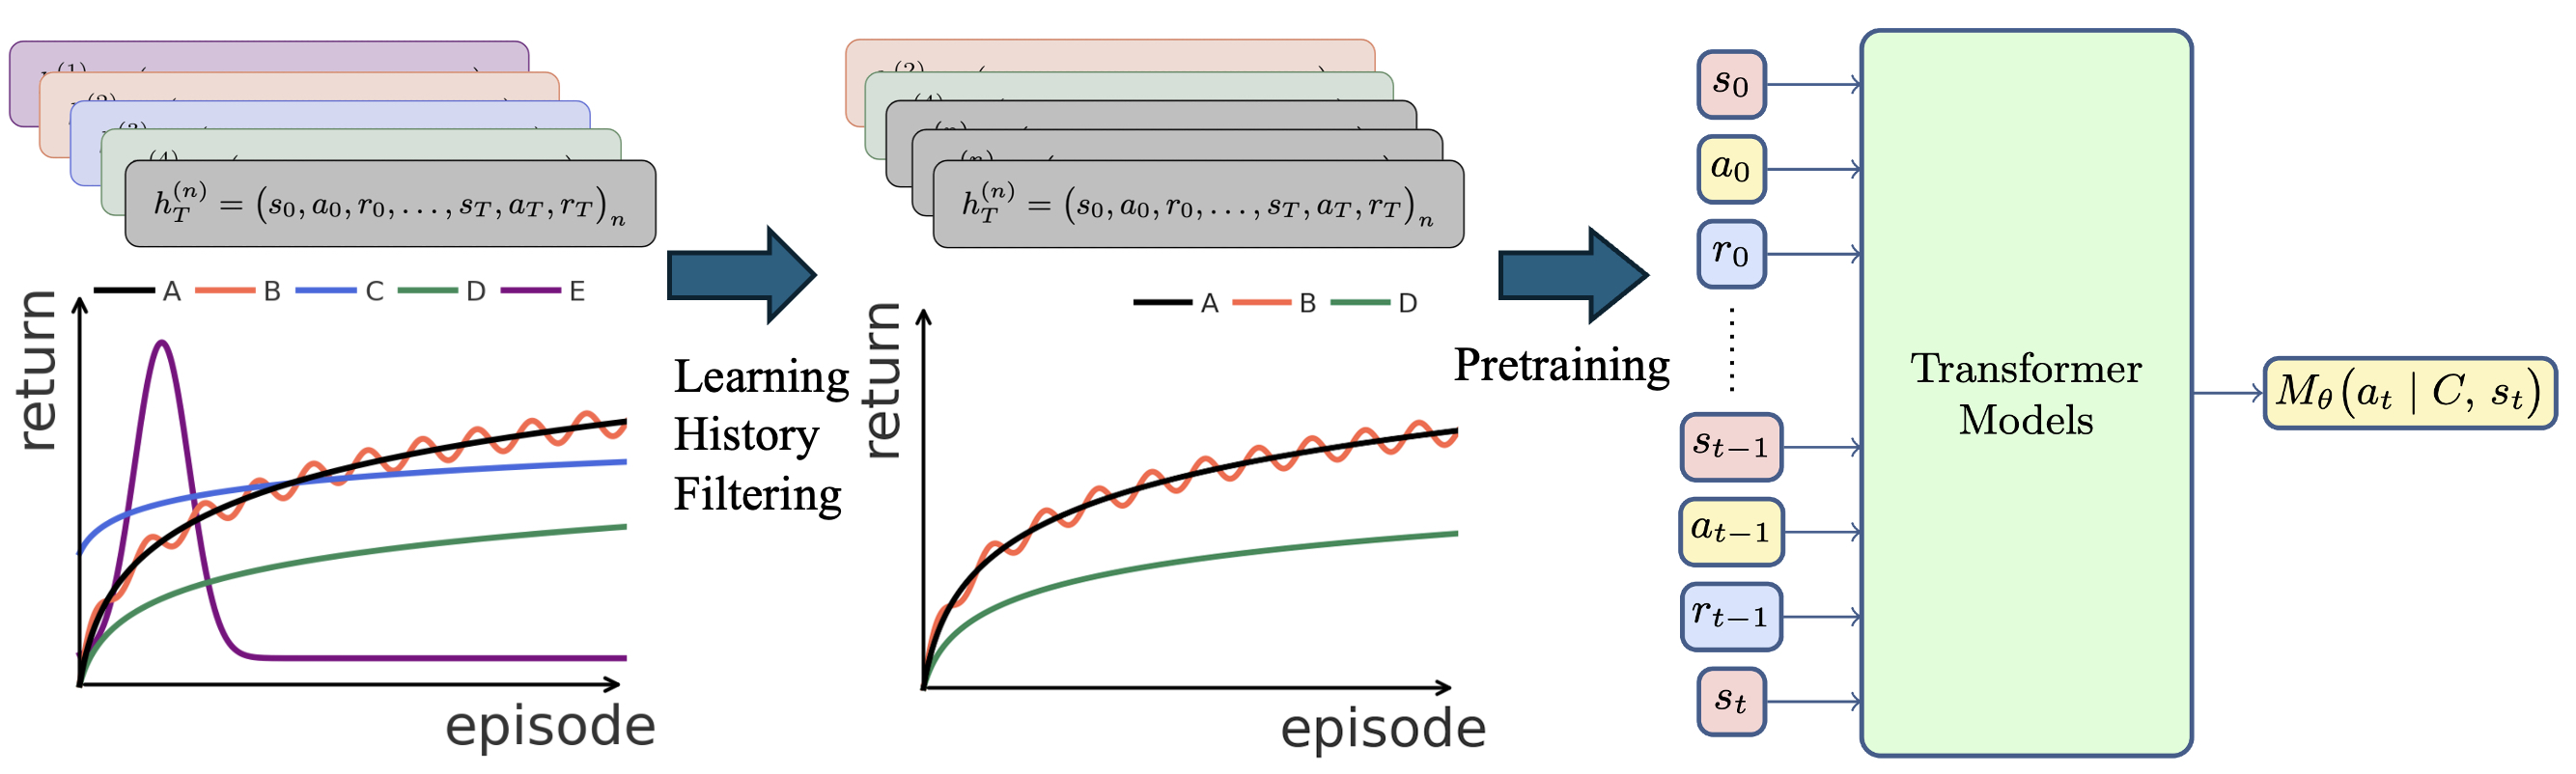
\includegraphics[width=\linewidth]{figures/learning_hist.jpg}
  \caption{The schematic of learning history filtering (LHF). Current ICRL methods employ a source RL algorithm (e.g., PPO) to collect the learning histories across a substantial amount of environments, resulting in a pretraining dataset composed of multiple learning histories with varying levels of performance (\textit{left}). 
  %
  LHF filters such pretraining dataset and randomly retains each learning history with different probabilities that depend on the improvement and stability characteristics inherent in the learning histories. As a result, high-quality learning histories (A, B, D) are more likely to be retained with varying proportions, while suboptimal ones (C, E) tend to be filtered out (\textit{middle}).
  %
  After filtering learning histories, we follow the standard process for pretraining transformer models (\textit{right}).
    }
  \label{fig_lhf_schematic}
\end{figure}




\textbf{Main Contributions.} $(i)$ We propose a novel approach of learning history filtering (LHF) to enhance ICRL, which, to the best of our knowledge, is the first method that addresses the issue of inheriting the source suboptimality from the perspective of dataset preprocessing (filtering).
%
$(ii)$ We substantiate the efficacy of LHF on multiple popular ICRL benchmark environments, including the discrete environments like \textit{Darkroom}-type problems and continuous robotic manipulation tasks, i.e., \textit{Meta-World-ML1}.
%
Our empirical results demonstrate that LHF consistently outperforms the original baselines without learning history filtering across all backbones algorithms and problems. In certain problems, such as \textit{Reach-Wall} in \textit{Meta-World-ML1}, our LHF approach outperforms the baselines by achieving over a $141\%$ performance enhancement.
%
$(iii)$ We further validate the robustness of LHF across multiple suboptimal scenarios such as noisy dataset, partial learning histories, and lightweight models, as well as with respect to the hyperparameter variations and different sampling strategies.











%
%
\section{Related Work}
\label{section_related_work}


\textbf{Transformer Models for RL.}
%
TMs~\citep{vaswani2017attention} have been successfully applied to offline RL by their promising capability in sequential modeling. The pioneering works include Decision Transformer~\cite{chen2021decision}, Trajectory Transformer~\cite{janner2021offline}, etc. Specifically, TMs autoregressively model the sequence of actions from the historical offline data conditioned on the sequence of returns in the history.
%
%
During the test, the trained model can be queried based on pre-defined target returns, allowing it to generate actions aligned with the target returns.
%
%
In addition, Multi-Game Decision Transformer (MGDT)~\citep{lee2022multi} and Gato~\citep{reed2022generalist} have exhibited the success of the autoregressive TMs in learning multi-task policies by fine-tuning or leveraging expert demonstrations in downstream environments. However, they suffer from poor zero-shot generalization and inferior in-context learning capabilities.








% \red{
% \subsection{Reducing Data Needs for ICRL}
% %
% The SOTA ICRL algorithms including AD~\citep{laskin2022context} and DPT~\citep{lee2024supervised} have demonstrated the potential of the ICRL framework. Nevertheless, both methods impose strict requirements on the pretraining dataset, e.g., requiring well-trained (or even optimal) behavior policies, which significantly restrict their practicality in real-world applications.
% %
% Under this circumstance, AD$^\epsilon$~\blue{[REF]} proposes to probabilistically infuse noises into the oracle or well-trained policies and to gradually decrease the probability of noises after each step, thus resembling the learning process from completely random policies to the final oracle/well-trained policies. On the other hand, DIT~\blue{[REF]} follows a DPT fashion except for selecting the query state and action label from the context dataset and prioritizing the training of the TMs on the state-action pairs with high return-to-go. However, DIT still mandates that more than $30\%$ of the context data comes from well-trained policies to ensure the coverage of good action labels. In this sense, SAD~\blue{[REF]} proposes to perform ICRL solely using random policies, by exploring and distilling the outstanding state and action pairs within a trust horizon.
% }






\textbf{In-Context Reinforcement Learning.}
%
%
The pioneering contributions in the field of ICRL include AD~\cite{laskin2022context} and DPT~\cite{lee2024supervised}, where the former imitates the complete learning histories of a source RL algorithm over a substantial amount of pretraining environments to distill the policy improvement operator, and the latter pretrains a TM to infer the target MDP from the surrounding context (can be derived from the learning history) and to take actions according to the optimal policy for the inferred target MDP.
%
%
% \red{Despite promising performance, the current SOTA ICRL methods~\cite{laskin2022context, lee2024supervised, huang2024incontext} tend to inherit the suboptimal behaviors of the source RL algorithm as they either imitate the entire learning histories of the source and/or consider the histories as the context.}\blue{In the intro} 
%
%
Although prior work~\cite{son2025distilling} has explored in-context model-based planning to address source suboptimality, it falls short of fully resolving the issue. On the other hand, recent studies~\cite{zisman2024emergence, dong2024context, chen2025random} consistently demonstrate that the performance of ICRL remains highly sensitive to the pretraining dataset.
%
Therefore, our work aims to address the issue of inheriting the source suboptimality from the perspective of dataset preprocessing.






\textbf{Weighted Empirical Risk Minimization.}
%
It is worth noting that ICRL follows a supervised pretraining mechanism~\cite{chen2025random}, which essentially undergoes an ERM process~\cite{bartlett2005local, massart2006risk}.
%
ERM identifies an optimal hypothesis from a hypothesis class that minimizes the empirical risk given a set of (input, label) samples. \cite{zhang2025reweighting} presents a WERM schema that exhibits provably improved excess risk bounds on ``high confidence'' regions than that of standard ERM. These ``high confidence'' regions could be large-margin regions in classification tasks and low-variance regions in heteroscedastic bounded regression problems~\cite{zhang2025reweighting}. Motivated by the superior performance of WERM over the standard ERM, we propose to preprocess (filter) the ICRL pretraining dataset by emulating a WERM schema, combined with crucial aspects in the ICRL like the improvement and stability of the learning histories.





%%%%%%%%%%%%%%%%%%%%%%%%%%%%%%%%%%%%%%%%%%%%%%%%%%%%%%%%%%%%%%%%%%%%%%%%


\section{In-Context Reinforcement Learning}
\label{section_preliminary}




% \subsection{Reinforcement Learning as a solution for Markov Decision Processes}

\textbf{RL Preliminaries.}
%
RL is a data-driven solution to MDPs~\citep{sutton2018reinforcement}. 
An MDP can be represented by a tuple $\tau = (\mbS, \mbA, R, P, \rho)$, where $\mbS$ and $\mbA$ denote state and action spaces, $R: \mbS \times \mbA \to \Real$ denotes the reward function that evaluates the quality of the action, $P: \mbS \times \mbA \times \mbS \to [0, 1]$ denotes the transition probability that describes the dynamics of the system, and $\rho: \mbS \to [0, 1]$ denotes the initial state distribution.  
%
A policy $\pi$ defines a mapping from the states to the probability distributions over the actions, providing a strategy that guides the agent in the decision-making.
%
The agent interacts with the environment following the policy $\pi$ and the transition dynamics of the system, and then generates a learning history $(s_0, a_0, r_0, s_1, a_1, r_1, \cdots)$.
%
The performance measure $J (\pi)$ is defined by the expected discounted cumulative reward under the policy $\pi$
\begin{align}
    J (\pi) = \mbE_{s_0 \sim \rho, a_t \sim \pi(\cdot | s_t), s_{t+1} \sim P(\cdot|s_t, a_t)} \left[ \sum_{t=0}^\infty \gamma^t r_t \right].
\end{align}
%
The goal of RL is to identify an optimal policy $\pi^\star$ that maximizes $J (\pi)$.
%
It is crucial to recognize that $\pi^\star$ often varies across different MDPs (environments). Accordingly, the optimal policy for standard RL must be re-learned each time a new environment is encountered.
%
%
To overcome this limitation, ICRL pretrains a TM on a wide variety of environments, and then deploys it in the \textit{unseen} test environments without updating the parameters of the TM, i.e., zero-shot generalization~\citep{sohn2018hierarchical, mazoure2022improving, zisselman2023explore, kirk2023survey}.






%%%%%%%%%%%%%%%%%%%%%%%%%%%%%%%%%%%%%%%%%%%%%%%%%%%%%%%%%%%%%%%%%%%%%%%%

\textbf{Supervised Pretraining of ICRL.}
%
%\blue{The notation in this section is not consistent. Sometimes regular letters are used for sets, sometimes $\mathbb{E}$. Caligraphic letters are the context and also the model. Let's work on this section and the previous one to make this more streamlined. } \purple{Weiqin: modified. Now, we use \textbf{Bold} for space, \textbf{Caligraphic} for distributions, datasets, collections, \textbf{Uppercase} letter for Models and general functions.}
%
%
Consider two distributions over the environments $\ccalT_{\text{pretrain}}$ and $\ccalT_{\text{test}}$ for pretraining and test. Each environment, along with its corresponding MDP $\tau$, can be regarded as an instance drawn from the environment distributions, where each environment may exhibit distinct reward functions and transition dynamics. Given an environment $\tau$, a context $\ccalC = \{s_i, a_i, r_i\}_{i \in [n']}$ refers to a collection of interactions between the agent and the environment $\tau$, sampled from a context distribution $\ccalD_{\text{pretrain}} (\cdot \mid \tau)$, i.e., $\ccalC \sim \ccalD_{\text{pretrain}} (\cdot \mid \tau)$. Notably, $\ccalD_{\text{pretrain}} (\cdot \mid \tau)$ contains the contextual information regarding the environment $\tau$.
We next consider a query state distribution $\ccalD_q^\tau$ and a label policy that maps the query state $s_q$ to the distribution of the action label $a_l$, i.e., $\pi_{l}: \mbS \to \Delta_{a_l} (\mbA)$. 
The joint distribution over the environment $\tau$, context $\ccalC$, query state $s_{q}$, and action label $a_{l}$ is given by
\begin{align}\label{eqn_pretrain_distribution}
    \ccalP_{\text{pretrain}} (\tau, \ccalC, s_{q}, a_{l}) = \ccalT_{\text{pretrain}} (\tau) \cdot \ccalD_{\text{pretrain}} (\ccalC | \tau) \cdot \ccalD_q^\tau \cdot \pi_{l}(a_{l} | s_{q}).
\end{align}
%
The supervised pretraining schema of ICRL is embodied in the process where a TM parameterized by $\theta$ (denoted as $M_\theta: \mbC \times \mbS \to \Delta(\mbA)$ is pretrained to predict the action label $a_l$ given the context $\ccalC$ and the query state $s_q$. To this end, current ICRL methods~\citep{laskin2022context, lee2024supervised, chen2025random, son2025distilling} consider a common objective
%
\begin{align}\label{eqn_icrl_obj_unweighted}
    \theta^\star = \argmin_\theta \mbE_{\ccalP_{\text{pretrain}}} \left[ l \left( M_\theta(\cdot \mid \ccalC, s_{q}), a_{l}\right) \right],
\end{align}
%
where $l(\cdot, \cdot)$ represents the loss function, e.g., $l \left( M_\theta(\cdot \mid \ccalC, s_{q}), a_{l}\right) = -
\log M_\theta(a_l \mid \ccalC, s_{q})$. 
%
% \blue{I think you should use this equation to point out the source suboptimality issue.}

It is crucial to highlight that, in the context of this work, $\ccalP_{\text{pretrain}}$ describes the distribution of learning histories. While the general problem of ICRL assumes a generic distribution, in this work, the context, query state and action label are obtained from the learning histories of an RL algorithm, e.g., PPO.


% for instance, negative log-likelihood (NLL) for discrete-action problems and mean square error (MSE) {\color{red}{for continuous-action scenarios.} }
%
% {\color{blue} {If we are considering continuous state-actions, the definition of the MDP is not correct. }}
% %
% \orange{Weiqin: The MDP definition above (discrete version) is more popular in the AI community. I would like to keep that. We can remove the red text.} {\color{blue}{I'm good with this option.}}



%%%%%%%%%%%%%%%%%%%%%%%%%%%%%%%%%%%%%%%%%%%%%%%%%%%%%%%%%%%%%%%%%%%%%%%%




\section{Learning History Filtering}
\label{section_LHF}


This section presents our dataset preprocessing approach, learning history filtering (LHF; summarized in Algorithm~\ref{alg_lhf}), which is inspired by the success of WERM~\cite{zhang2025reweighting} and the fact that ICRL adheres to a supervised pretraining paradigm. Specifically, WERM demonstrates that reweighting the training objective based on appropriate metrics can lead to provable performance enhancement.
%
In the remainder of this section, we start by presenting a weighted learning history sampling mechanism for ICRL that emulates the WERM schema. Following that, we formally define the metrics used in the weighted sampling that play important roles in the pretraining of ICRL (supported by our empirical evidence in Section~\ref{section_experiment}). Lastly, we describe specific sampling strategies based on these metrics that are equivalent to weighting the learning histories.







\textbf{Weighted Sampling for ICRL.}
%
%\blue{same comments regarding notation as before. Instead of having this here, I would make the introduction of section 4 a bit longer to include the weighted ERM using the notation of ICRL. That could even be section 4.1. } \blue{You don't need to rewrite (3). What I suggest is that you replace (5) with (6) or (7).} \purple{Weiqin: modified.}
%
% Consider a set of independent and identically distributed (i.i.d.) data samples $\ccalS_n = \{\bbd_i  \mid \bbd_i := (\bbx_i, y_i)\}_{i=1}^n$, where $\bbx_i$ and $y_i$ denote the input (e.g., feature vector) and the corresponding label in the supervised learning problems, respectively. The goal of ERM is to identify a hypothesis $f$ in a hypothesis class $\ccalF$ that minimizes the empirical risk over the set of samples $\ccalS_n$, i.e., 
% %
% \begin{align}\label{eqn_ERM}
%     f_\text{ERM} := \argmin\limits_{f \in \ccalF} \, \frac{1}{n} \sum_{i=1}^n l(f, \bbd_i),
% \end{align}
% %
% where $l(\cdot, \cdot)$ represents the loss (risk) function.
% which may take the form $l(f, \bbd_i) = (f(\bbx_i) - y_i)^2$ in regression problems or $l(f, \bbd_i) = \mathbbm{1} (f(\bbx_i) \neq y_i)$ in classification tasks.
%
%
% Denote by $f^\star$ the optimal hypothesis in $\ccalF$ such that $f^\star := \argmin_{f \in \ccalF} \,\mbE_\bbd \left[ l(f, \bbd)\right]$. We then define the excess risk of any hypothesis $f$ by $\mbE_\bbd \left[ l(f, \bbd)\right] - \mbE_\bbd \left[ l(f^\star, \bbd)\right]$.
%
%
WERM~\cite{zhang2025reweighting} leverages a problem-dependent weighted structure to improve upon ERM. Concretely, an input-dependent weight function $w(\cdot)$ is employed to re-weight the ERM objective. In the case of ICRL, the new weighted objective function based on \eqref{eqn_icrl_obj_unweighted} is given by
%
\begin{align}\label{eqn_icrl_obj_weighted_train}
    \theta_w^\star = \argmin_\theta \mbE_{\ccalP_{\text{pretrain}}} \left[ w(\tau, \mathcal{C}, s_q, a_l) \cdot l \left( M_\theta(\cdot \mid \ccalC, s_{q}), a_{l}\right) \right],
\end{align}
%
where the weight $w$ relies on the environment $\tau$, context $\ccalC$, query state $s_q$, and action label $a_l$, and is essentially determined by the learning history.
%
%
To emulate the WERM schema during the dataset preprocessing, we adopt a random sampling strategy guided by the learning history. In particular, we define $\bar{w}$ to be the random variables taking the values $0$ or $1$ according to a distribution that we denote by $\mathcal{P}_{\bar{w}}(\tau,\mathcal{C},s_q,a_l)$ (see e.g., \eqref{eqn_linear_weight_func}). Subsequently, by defining a new learning history distribution $\ccalP_{\text{pretrain}}^w = \mathcal{P}_{\bar{w}}(\tau, \mathcal{C}, s_q, a_l) \cdot \ccalP_{\text{pretrain}} (\tau, \ccalC, s_{q}, a_{l})$, we adopt the following objective
\begin{align}\label{eqn_icrl_obj_weighted_data}
    \theta_w^\star = \argmin_\theta \mbE_{\ccalP_{\text{pretrain}}^w} \left[ l \left( M_\theta(\cdot \mid \ccalC, s_{q}), a_{l}\right) \right].
\end{align}
%
Notice that for any set of weights in \eqref{eqn_icrl_obj_weighted_train} between $0$ and $1$, it is always possible to define a probability distribution $\mathcal{P}_{\bar{w}}(\tau,\mathcal{C},s_q,a_l)$ such that \eqref{eqn_icrl_obj_weighted_data} becomes equivalent to  \eqref{eqn_icrl_obj_weighted_train}.






%
% \begin{proposition}[\cite{zhang2025reweighting}]
%     In classification tasks, denote by $f$ the hypothesis estimator obtained from ERM or WERM. ERM and WERM achieve the same excess risk bound as follows
%     \begin{align}
%         \mbE_\bbd \left[ \mathbbm{1} (f(\bbx) \neq y) - \mathbbm{1} (f^\star(\bbx) \neq y) \right] \leq  \frac{\epsilon}{\gamma}.
%     \end{align}
% \end{proposition}


% \begin{proposition}[\cite{zhang2025reweighting}]
%     In heteroscedastic bounded regression problems, denote by $f$ the hypothesis estimator obtained from ERM or WERM. ERM and WERM achieve the same excess risk bound as follows
%     \begin{align}
%         \mbE_\bbd \left[ (f(\bbx) - y)^2 - (f^\star(\bbx) - y)^2 \right] \leq \frac{\epsilon}{\gamma^2}.
%     \end{align}
% \end{proposition}



% For \blue{sub-regions, e.g., large-margin regions in classification tasks and low-variance regions in heteroscedastic bounded regression problems}, WERM achieves improved excess risk bounds than that of standard ERM. We formalize this in the next two theorems.

% \begin{theorem}[\cite{zhang2025reweighting}]
%     In classification tasks, denote by $f_\text{ERM}$ and $f_\text{WERM}$ the hypothesis estimators obtained from ERM and WERM, respectively. For large margin region such that $w^\star (\bbx) > c$ where $w (\bbx) := 2P(y=f^\star (\bbx) | \bbx) - 1$ and $c > \gamma$ is a constant. ERM and WERM achieve the following excess risk bounds, respectively
%     \begin{align}
%         &\mbE_\bbd \left[ \mathbbm{1} (f_\text{ERM}(\bbx) \neq y) - \mathbbm{1} (f^\star(\bbx) \neq y) \right] \leq  \frac{\epsilon}{\gamma} \frac{1}{P(w (\bbx) > c)} \\
%         &\mbE_\bbd \left[ \mathbbm{1} (f_\text{WERM}(\bbx) \neq y) - \mathbbm{1} (f^\star(\bbx) \neq y) \right] \leq  \frac{\epsilon}{c} \frac{1}{P(w (\bbx) > c)}
%     \end{align}
% \end{theorem}




% \begin{theorem}[\cite{zhang2025reweighting}]
%     In heteroscedastic bounded regression problems, denote by $f_\text{ERM}$ and $f_\text{WERM}$ the hypothesis estimators obtained from ERM and WERM, respectively. For low-variance regions such that $\sigma^2(\bbx) < 1/c$ where $w (\bbx) := 1 / \sigma^2(\bbx)$ and $c > \gamma$ is a constant. ERM and WERM achieve the following excess risk bounds, respectively
%     \begin{align}
%         &\mbE_\bbd \left[ (f_\text{ERM}(\bbx) - y)^2 - (f^\star(\bbx) - y)^2 \right] \leq \frac{\epsilon}{\gamma^2} \frac{1}{P(\sigma^2(\bbx) < 1/c)} \\        &\mbE_\bbd \left[ (f_\text{WERM}(\bbx) - y)^2 - (f^\star(\bbx) - y)^2 \right] \leq \frac{\epsilon}{\gamma c} \frac{1}{P(\sigma^2(\bbx) < 1/c)} \\
%     \end{align}

    
    
% \end{theorem}

























\textbf{Improvement and Stability of Learning Histories.}
%
%
%{\color{blue}{Shouldn't the learning history include also the states and actions? For the computation of the metric, we only care about the returns, but when you add it to the set $D_{LHF}$, you need the states and the actions too. What's the difference between $\mathcal{D}_i$ and the learning history?}}
%{\color{blue}{I'm not very happy with how this section is written. It's not formal enough.}}  \purple{Weiqin: modified.}
%
%
The weight in the WERM is crafted to reflect key aspects of the training process, such as the improvement and stability characteristics inherent in learning trajectories as exemplified by ICRL~\cite{laskin2022context, zisman2024emergence}.
%
To formalize the improvement and stability, we define a learning history as the collection of state-action-reward tuples $(s, a, r)$ generated during a single run of a source RL algorithm (e.g., PPO) within a single environment. Since each environment may yield multiple learning histories, we denote by $\ccalD_i^l$ the $l$-th learning history in the $i$-th environment.
%
Then, we define the improvement of a learning history $\ccalD_i^l$ with respect to its episodic returns %as follows
%
\begin{align}
    \texttt{Improvement}(\ccalD_i^l) = \frac{\bar{R}(\ccalD_i^l) + R_G(\ccalD_i^l)}{2 R_\text{max}^i}, 
\end{align}
%
where $R_\text{max}^i$ denotes the maximum episodic return available in the $i$-th environment, $\bar{R}(\ccalD_i^l)$ represents the mean of episodic returns in the learning history $\ccalD_i^l$, and $R_G(\ccalD_i^l)$ denotes the difference (gap) between the maximal and minimal episodic returns in the learning history $\ccalD_i^l$. Note that the \texttt{Improvement} metric takes a value in $[0, 1]$.


To quantify the stability of a learning history, we consider the sequence of episodic returns within $\ccalD_i^l$ and compute the difference between each return and its immediate successor. We then extract the negative differences, indicating performance degradations, and compute their mean. This measure is denoted by $\bar{R}_D(\ccalD_i^l)$. Subsequently, we define the stability of the learning history $\ccalD_i^l$ by
%
\begin{align}
    \texttt{Stability}(\ccalD_i^l) = 1 + \frac{\bar{R}_D(\ccalD_i^l)}{R_\text{max}^i},
\end{align}
%
where the $\texttt{Stability}$ metric takes a value in the range $[0, 1]$ as well.
%
Having formalized the improvement and stability, we integrate them into a unified metric
\begin{align}\label{eqn_metric}
    U(\ccalD_i^l) = \texttt{Improvement}(\ccalD_i^l) + \lambda \cdot \texttt{Stability}(\ccalD_i^l),
\end{align}
%
where $\lambda$ is a hyperparameter that trades-off the improvement and stability. Indeed, for large values of $\lambda$ the unified metric $U(\ccalD_i^l)$ will prioritize the stability in the learning history, whereas for small values of $\lambda$ the metric will focus on the improvement. Section~\ref{section_sensitivity} demonstrates the robust performance of our LHF approach with respect to various choices of $\lambda$. As depicted in Figure~\ref{fig_lhf_schematic}, $U(\ccalD_i^l)$ encapsulates important characteristics in the learning history that play crucial roles in the pretraining of TMs.











\textbf{Sampling Strategy.}
%
Having defined the unified metric $U(\ccalD_i^l)$, we are now in the stage of introducing the sampling strategy that allows us to emulate the WERM scheme during the dataset preprocessing.
%
%
\begin{algorithm}
\caption{Learning History Filtering (LHF)}         
\label{alg_lhf}
\begin{algorithmic}[1]

        \STATE \textbf{Require:} Pretraining dataset $\{\ccalD_i^l\}$ with $i \in [N_i], l \in [N_l]$, empty LHF dataset $\ccalD_\text{LHF}$

        \FOR{$i$ in $[N_i]$}

            \STATE Let $\ccalD_i' = \emptyset$
            \WHILE{$|\ccalD_i'| < |\ccalD_i|$}
                    
                \FOR{$l$ in $[N_l]$}

                    \STATE Compute the unified metric $U(\ccalD_i^l)$ by \eqref{eqn_metric}
                    \STATE Compute the weighted probability $\mathcal{P}_{\bar{w}}(U(\ccalD_i^l))$ for the learning history $\ccalD_i^l$ by \eqref{eqn_linear_weight_func}
                    \STATE Sample a uniform random variable $v \sim \ccalU[0, 1]$
                    \STATE Add the learning history $\ccalD_i^l$ to $\ccalD_i'$ \textbf{if} $v \leq \mathcal{P}_{\bar{w}}(U(\ccalD_i^l))$
                    \IF{$|\ccalD_i'| = |\ccalD_i|$}
                    \STATE break
                    \ENDIF
                \ENDFOR
            \ENDWHILE
 
            \STATE $\ccalD_\text{LHF} \leftarrow \ccalD_\text{LHF} \cup \ccalD_i'$
        \ENDFOR
        
        \STATE \textbf{Return} $\ccalD_\text{LHF}$
\end{algorithmic}
\end{algorithm}
%
%

Given a static pretraining dataset $\{\ccalD_i^l\}$, where $i \in [N_i]$ indexes environments and $l \in [N_l]$ indexes learning histories within each environment, we construct an empty dataset $\ccalD_{\text{LHF}}$ for filtering the learning history. For each learning history $\ccalD_i^l$, we define a weighted sampling probability that depends linearly on its unified metric $U(\ccalD_i^l)$
%
\begin{align}\label{eqn_linear_weight_func}
    \mathcal{P}_{\bar{w}}(U(\ccalD_i^l)) = \frac{U(\ccalD_i^l) - \min_{l \in [N_l]} U(\ccalD_i^l)}{\max_{l \in [N_l]} U(\ccalD_i^l) - \min_{l \in [N_l]} U(\ccalD_i^l)}.
\end{align}
%
%
Guided by \eqref{eqn_icrl_obj_weighted_data}, we in turn randomly select the learning histories in $\{\ccalD_i^l\}$ with the corresponding weighted probability $\mathcal{P}_{\bar{w}}(U(\ccalD_i^l))$ for each learning history in each environment, and add it to our LHF dataset $\ccalD_\text{LHF}$ until its size matches that of $\{\ccalD_i^l\}$. The procedure is detailed in Algorithm~\ref{alg_lhf}.
%
%
It is important to note that the linear sampling strategy \eqref{eqn_linear_weight_func} is not the only choice for our LHF approach. Other sampling strategies, such as Softmax, can also be employed. Section~\ref{section_sensitivity} demonstrates the robustness of LHF combined with Softmax sampling function with varying temperature parameters.


After preprocessing the dataset by LHF, we follow the standard processes for pretraining and testing TMs as in the ICRL literature~\cite{laskin2022context, lee2024supervised, chen2025random}, which are outlined in Algorithm~\ref{alg_whole} in Appendix~\ref{append_complete_pseudocode}.





\section{Experiments}
\label{section_experiment}


We substantiate the efficacy of our LHF approach across a diverse set of environments, which are commonly considered in ICRL literature~\citep{laskin2022context, lee2024supervised, son2025distilling, chen2025random}.
%
These environments include discrete settings such as \textit{Darkroom, Darkroom-Permuted, Darkroom-Large, Dark Key-to-Door} and continuous robotic manipulation tasks from the \textit{Meta-World-ML1} benchmark like \textit{Reach, Reach-Wall, Button-Press, Basketball, Door-Unlock, Push, Soccer, Hand-Insert}.
%
All these problems are challenging to solve in-context, as the test environments differ from the pretraining environments, while the parameters of the TM remain frozen during the test. The environmental setup is detailed in Appendix~\ref{append_env_setup}.







\subsection{Collecting and Filtering Learning Histories}
\label{subsec_collect_filter_hist}

Following previous ICRL works~\cite{laskin2022context, son2025distilling}, we consider PPO as the source RL algorithm to collect learning histories in the \textit{Darkroom}-type and \textit{Meta-World-ML1} problems. As introduced in Appendix~\ref{append_env_setup}, each problem includes multiple distinct environments depending on e.g., the goal locations. For each environment, we employ $100$ PPO agents to collect $100$ learning histories with each comprising $1000$ transitions for \textit{Darkroom}-type and $10,000$ transitions for \textit{Meta-World-ML1}. This yields a total of $100,000$ transitions per \textit{Darkroom}-type environment and $1,000,000$ transitions per \textit{Meta-World-ML1} environment. We provide the detailed procedure of collecting learning histories in Appendix~\ref{append_collect_history}.
%
%
Having collected the pretraining dataset of learning histories, we next filter the dataset by LHF, which is detailed in Section~\ref{section_LHF} and summarized in Algorithm~\ref{alg_lhf}.






\subsection{Backbone ICRL Algorithms}


Since our LHF approach exclusively targets the dataset preprocessing, it can be seamlessly integrated with various backbone algorithms to enable ICRL.
%
In this work, we adopt three SOTA ICRL algorithms (AD, DICP, DPT) as the backbones, each employing distinct strategies to learn from the pretraining dataset of learning histories. More details of the backbone ICRL algorithms are presented in Appendix~\ref{append_backboneICRLalgo}.
%
%
Same as in the DICP paper~\cite{son2025distilling}, we assess AD and DICP across all environments introduced in Appendix~\ref{append_env_setup} and evaluate DPT only within the four \textit{Darkroom}-type environments, as DPT relies on the optimal action labels that are typically unavailable in more general environments such as \textit{Meta-World-ML1}.
%
%
In addition, since all backbone ICRL algorithms are transformer-based, we consider the same transformer architecture (TinyLlama~\cite{zhang2024tinyllama}) across all experiments to ensure a fair comparison. The transformer hyperparameters, such as the number of attention layers, the number of attention heads, the embedding dimension etc, are detailed in Appendix~\ref{append_transformer_hyperparameter}.



\subsection{Numerical Results}
\label{exp_numerical_result}

\begin{wraptable}{r}{0.5\textwidth}
    \centering
    \caption{Relative enhancement (\%) of LHF over baselines. Backbone algorithms: AD, DICP, DPT.}
    \label{tab_darkrooms_OriginaData_FullHistory}
    \begin{tabular}{cccc}    
        \toprule
        Task & AD & DICP & DPT \\
        \midrule
        \textit{DarkRoom} & \textbf{25.1} & 15.2 & 3.5 \\
        \textit{Darkroom-Permuted} & 5.0 & \textbf{9.2} & 2.6 \\
        \textit{Darkroom-Large} & 3.2 & 9.3 & \textbf{26.1} \\
        \textit{Dark Key-to-Door} & 1.8 & 2.5 & \textbf{15.5} \\
        \midrule
        Average & 8.8 & 9.1 & \textbf{11.9} \\
        \bottomrule
    \end{tabular}
    \vspace{-5pt}
\end{wraptable}



We first exhibit the enhanced performance of our LHF approach by empirical evidence across the three SOTA backbone algorithms and the four \textit{Darkroom}-type environments. Then we move on to the experiments in suboptimal scenarios in terms of the noisy dataset, lightweight model, and partial learning histories, which consistently substantiate the robustness of LHF. Notably, the superiority of LHF becomes even more pronounced in the noisy scenario and across all suboptimal scenarios with AD as the backbone. 
%
To assess the overall performance of our LHF approach, we adopt the linear sampling strategy and fix the stability coefficient at $\lambda = 1$ across all experiments. That being said, we also examine the robustness of LHF in terms of the varying stability coefficient $\lambda$ and by exploring an alternative Softmax sampling strategy with a set of temperature parameters.
%
To quantify the relative enhancement of our LHF approach over the original backbone algorithms (baselines) in terms of the speed and final performance, we define the relative enhancement $E$ as $E = (\bar{R}(\text{LHF}) - \bar{R}(\text{baseline})) / \bar{R}(\text{baseline})$ where $\bar{R}(\cdot)$ denotes the mean of episodic returns during the test.




%%%%%%%%%%%%%%%%
\begin{figure}[ht]
\centering 
\setcounter{subfigure}{0}
\subfigure[Darkroom]
{
	\begin{minipage}{0.25\linewidth}
	\centering 
	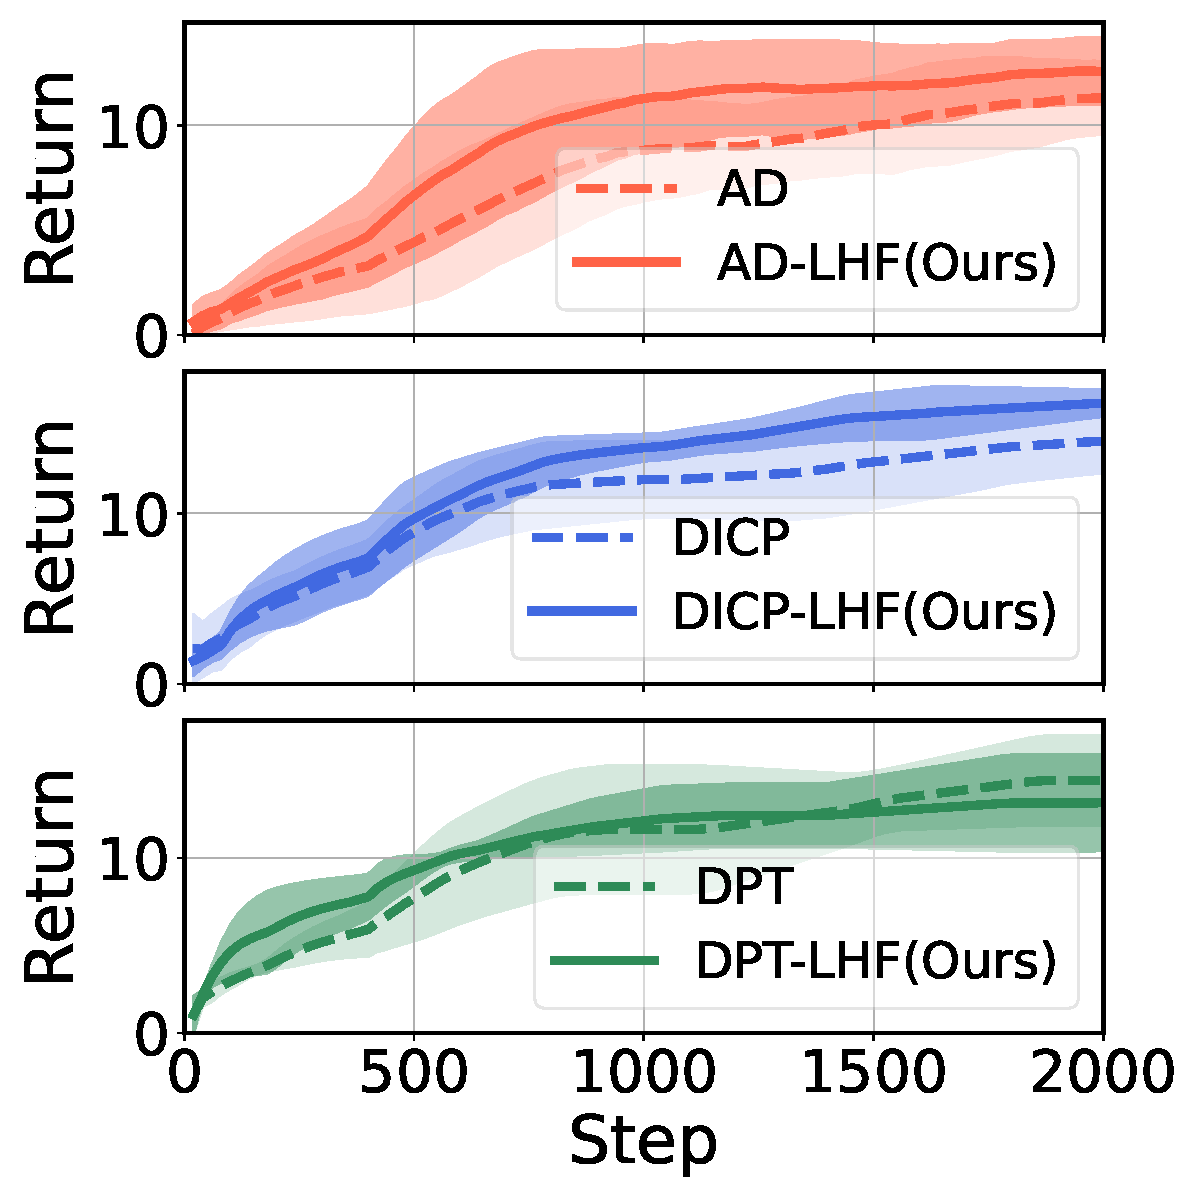
\includegraphics[width=1.0\columnwidth]{figures/DR_AD_DICP_OUR_AD_OUR_DICP.pdf}
	\end{minipage}
}
\!\!\!\!\!\!\!
\subfigure[Darkroom-Permuted]
{
	\begin{minipage}{0.25\linewidth}
	\centering 
	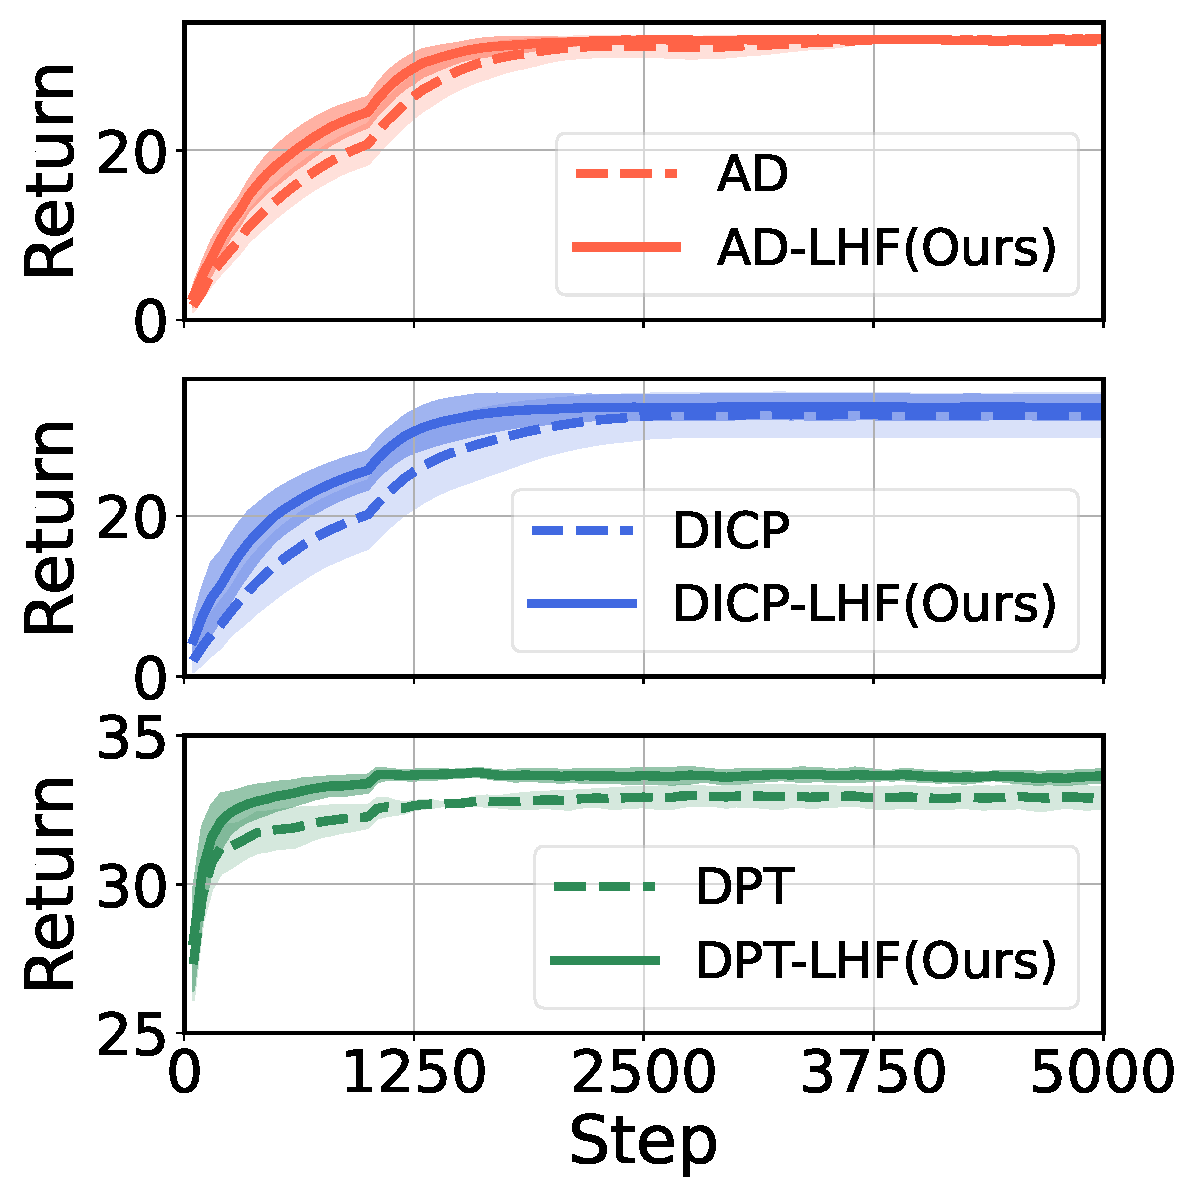
\includegraphics[width=1.0\columnwidth]{figures/DRP_AD_DICP_OUR_AD_OUR_DICP.pdf}
	\end{minipage}
}
\!\!\!\!\!\!\!
\subfigure[Darkroom-Large]
{
	\begin{minipage}{0.25\linewidth}
	\centering 
	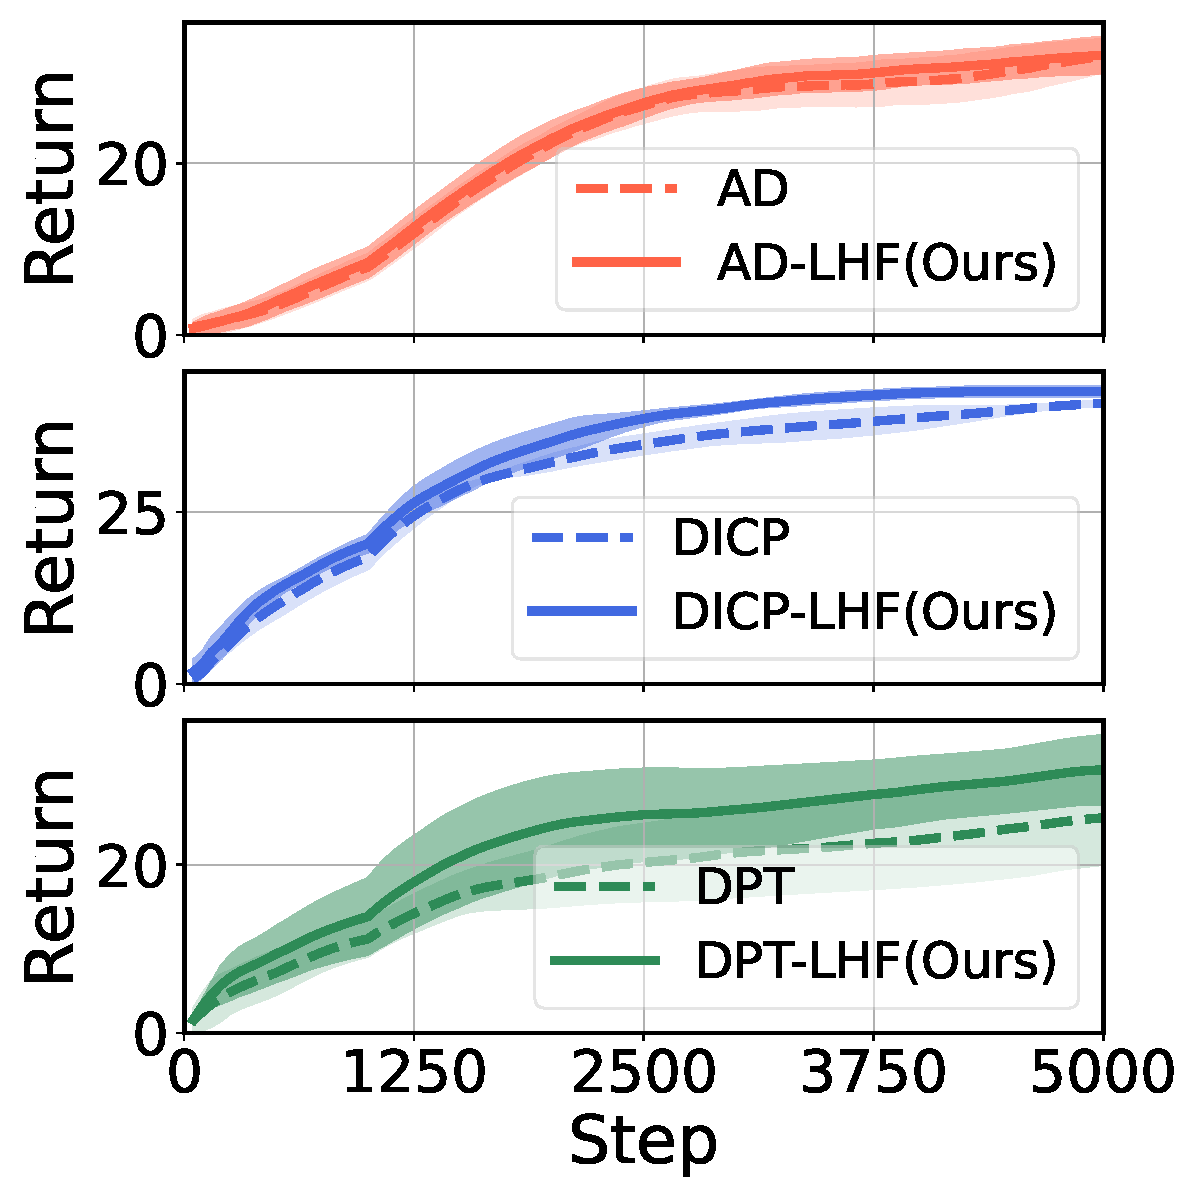
\includegraphics[width=1.0\columnwidth]{figures/DRL_AD_DICP_OUR_AD_OUR_DICP.pdf}
	\end{minipage}
}
\!\!\!\!\!\!\!
\subfigure[Dark Key-to-Door]
{
	\begin{minipage}{0.25\linewidth}
	\centering 
	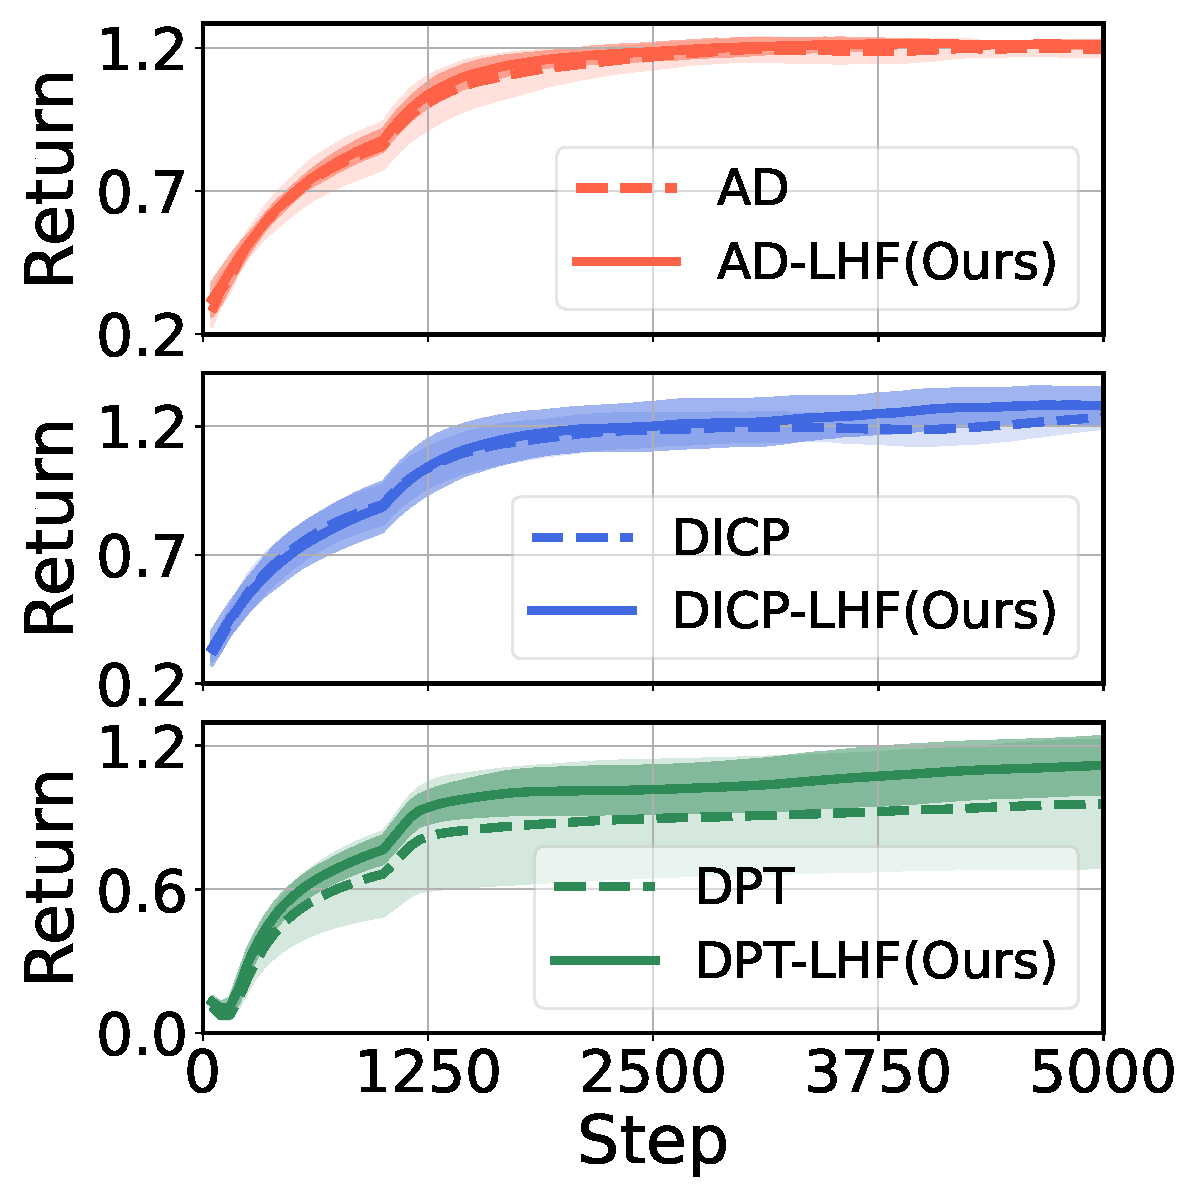
\includegraphics[width=1.0\columnwidth]{figures/DKTD_AD_DICP_OUR_AD_OUR_DICP.pdf}
	\end{minipage}
}
%
%
%
\caption{Learning curves of our LHF approach (solid lines) compared with original baselines (dashed lines) during the test. Each algorithm contains three independent runs with mean and standard
deviation. The backbone algorithms include AD (red), DICP (blue), and DPT (green).}
% optimal dataset + full learning history
\label{fig_darkrooms_OriginaData_FullHistory}
\end{figure}
%%%%%%%%%%%%%%%%




%%%%%%%%%%%%%%%%
\begin{wraptable}{r}{0.5\textwidth}
    \centering
    \vspace{-5pt}
    \caption{Relative enhancement (\%) of LHF over the baselines, provided with the noisy dataset.}
    \label{tab_darkrooms_NoisyDataset}
    \begin{tabular}{cccc}    
        \toprule
        Task & AD & DICP & DPT \\
        \midrule
      \textit{DarkRoom} & \textbf{90.7} & 19.0 & 21.4 \\
      \textit{Darkroom-Permuted} & 5.5 & \textbf{9.5} & 4.0 \\
      \textit{Darkroom-Large} & 13.8 & \textbf{17.3} & 13.9 \\
      \textit{Dark Key-to-Door} & 1.2 & 4.2 & \textbf{10.1} \\
     \midrule
      Average & \textbf{27.8} & 12.5 & 12.4 \\
        \bottomrule
    \end{tabular}
    \vspace{-5pt}
\end{wraptable}
%%%%%%%%%%%%%%%%




\textbf{Can LHF enhance ICRL?}
%
We collect the pretraining dataset as in Section~\ref{subsec_collect_filter_hist}, and implement the three backbone algorithms (AD, DICP, DPT) in four \textit{Darkroom}-type problems with and without LHF.
%
The numerical results are presented in Figure~\ref{fig_darkrooms_OriginaData_FullHistory} and Table~\ref{tab_darkrooms_OriginaData_FullHistory}.
%
All positive relative enhancement in Table~\ref{tab_darkrooms_OriginaData_FullHistory} implies the consistently improved performance of our LHF approach over the baselines across all backbone algorithms and problems. 
%
On average, AD, DICP, and DPT yield relative enhancement of $8.8\%$, $9.1\%$, and $11.9\%$, respectively. Notably, certain scenarios like using AD in \textit{Darkroom} and employing DPT in \textit{Darkroom-Large} can achieve more than $25\%$ performance enhancement.






\textbf{Can LHF enhance ICRL given a noisy dataset?}
%
To validate the robustness of our LHF approach and to assess the significance of filtering learning histories, we now inject noises into the pretraining dataset. Concretely, the learning histories in the dataset are collected by $70\%$ PPO agents and $30\%$ random agents (executing uniform random actions).
%
%
The numerical results are presented in Figure~\ref{fig_darkrooms_NoisyDataset} and Table~\ref{tab_darkrooms_NoisyDataset}.
%
All positive relative enhancement in Table~\ref{tab_darkrooms_NoisyDataset} implies the consistently improved performance of LHF over the baselines across all backbone algorithms and problems, provided with the noisy dataset. 
%
On average, AD, DICP, and DPT yield relative enhancement of $27.8\%$, $12.5\%$, and $12.4\%$, respectively. It is worth highlighting that the noisy dataset (see Table~\ref{tab_darkrooms_NoisyDataset}) achieves an increased average relative enhancement than the dataset without the noises (see Table~\ref{tab_darkrooms_OriginaData_FullHistory}). In certain scenarios, such as employing AD in \textit{Darkroom}, performance enhancement can even exceed $90\%$. These results provide compelling evidence supporting the importance of filtering learning histories.






%%%%%%%%%%%%%%%%
\begin{figure}[ht]
\centering 
\setcounter{subfigure}{0}
\subfigure[Darkroom]
{
	\begin{minipage}{0.25\linewidth}
	\centering 
	\includegraphics[width=1.0\columnwidth]{figures/Noise_darkroom_AD_DICP_OUR_AD_OUR_DICP.pdf}
	\end{minipage}
}
\!\!\!\!\!\!\!
\subfigure[Darkroom-Permuted]
{
	\begin{minipage}{0.25\linewidth}
	\centering 
	\includegraphics[width=1.0\columnwidth]{figures/Noise_darkroom_Permuted_AD_DICP_OUR_AD_OUR_DICP.pdf}
	\end{minipage}
}
\!\!\!\!\!\!\!
\subfigure[Darkroom-Large]
{
	\begin{minipage}{0.25\linewidth}
	\centering 
	\includegraphics[width=1.0\columnwidth]{figures/Noise_Large_darkroom_AD_DICP_OUR_AD_OUR_DICP.pdf}
	\end{minipage}
}
\!\!\!\!\!\!\!
\subfigure[Dark Key-to-Door]
{
	\begin{minipage}{0.25\linewidth}
	\centering 
	\includegraphics[width=1.0\columnwidth]{figures/Noise_darkkeytodoor_Permuted_AD_DICP_OUR_AD_OUR_DICP.pdf}
	\end{minipage}
}
%
%
%
\caption{Learning curves of our LHF approach (solid lines) compared with original baselines (dashed lines) during the test. Each algorithm contains three independent runs with mean and std., provided with the noisy dataset. The backbone algorithms include AD (red), DICP (blue), and DPT (green).}
\label{fig_darkrooms_NoisyDataset}
% datasets with 30% noise
\end{figure}
%%%%%%%%%%%%%%%%









\textbf{Can LHF enhance ICRL given partial learning histories?}
%
%
Current ICRL algorithms require learning from sufficient improvements in order to distill the underlying improvement operator within the algorithm. Therefore, we now evaluate our LHF approach under a more challenging setting where only partial learning histories are provided. We select the first half ($50\%$) of learning histories from each environment in each problem, forming a new dataset with half learning histories only.
%
The numerical results are presented in Figure~\ref{fig_darkrooms_half_learn_hist} and Table~\ref{tab_darkrooms_half_learn_hist} (see Appendix~\ref{append_addition_result_half_learn_hist}).
%
All positive relative enhancement in Table~\ref{tab_darkrooms_half_learn_hist} except for the case of using DPT in \textit{Darkroom-Permuted} implies the consistently improved performance of our LHF approach over the baselines across most backbone algorithms and problems, provided with half learning histories.
%
On average, AD, DICP, and DPT yield relative enhancement of $11.2\%$, $4.9\%$, and $8.3\%$, respectively. Interestingly, the average performance enhancement of AD using half learning histories (see Table~\ref{tab_darkrooms_half_learn_hist}) is slightly higher than that using the complete learning histories (see Table~\ref{tab_darkrooms_OriginaData_FullHistory}). The certain scenario like employing AD in \textit{Darkroom-Large} demonstrates more than $22\%$ relative performance enhancement.





%%%%%%%%%%%%%%%%%%%%%%%%%%%%%%%%%%%%%%

\begin{wraptable}{r}{0.31\textwidth}
    \centering
    \caption{Relative enhancement (\%) of LHF over baselines, provided with \textit{Meta-World-ML1}.}
    \label{tab_metaworld_ppo}
    \begin{tabular}{ccc}
    \toprule
    Task & AD & DICP \\
    \midrule
     \textit{Reach} & 2.4 & \textbf{64.6} \\
     \textit{Reach-Wall} & 5.9 & \textbf{141.3} \\
     \textit{Button-Press} & \textbf{13.4} & 2.4 \\
     \textit{Basketball} & 7.7 & \textbf{51.2} \\
     \textit{Door-Unlock} & 4.8 & \textbf{77.8} \\
     \textit{Push} & -0.4 & \textbf{18.9} \\
     \textit{Soccer} & \textbf{16.6} & 14.2 \\
     \textit{Hand-Insert} & \textbf{43.5} & -0.8 \\
     \midrule
     Average & 11.7 & \textbf{46.2} \\
    \bottomrule
    \end{tabular}
    \vspace{-5pt}
\end{wraptable}

%%%%%%%%%%%%%%%%%%%%%%%%%%%%%%%%%%%%%%




\textbf{Can LHF enhance ICRL given lightweight models?}
%
We further investigate the performance of LHF provided with lightweight models. 
%
Given the hyperparameters of TMs as presented in Appendix~\ref{append_transformer_hyperparameter}, we select four representative hyperparameters: the number of attention layers ($4$), the number of attention heads ($4$), the embedding dimension ($32$), the intermediate size ($128$), and reduce each by half yielding $(2, 2, 16, 64)$.
%
The numerical results are presented in Figure~\ref{fig_darkrooms_lightweight_model} and Table~\ref{tab_darkrooms_lightweight_model} (see Appendix~\ref{append_addition_result_lightweight_model}).
%
All positive enhancement in Table~\ref{tab_darkrooms_lightweight_model}, except for the case of using DPT in \textit{Darkroom-Permuted}, implies the consistently improved performance of LHF over the baselines across most backbone algorithms and problems, provided with lightweight models.
%
On average, AD, DICP, and DPT yield relative enhancement of $12.6\%$, $13.0\%$, and $4.2\%$. The certain scenario, e.g., using DICP in \textit{Darkroom}, exhibits more than $28\%$ performance enhancement. Notably, average performance enhancements of AD and DICP using lightweight models (see Table~\ref{tab_darkrooms_lightweight_model}) exceed those achieved with heavyweight models (see Table~\ref{tab_darkrooms_OriginaData_FullHistory}), suggesting the possibility of overfitting in the latter.










%%%%%%%%%%%%%%%%
\begin{figure}[ht]
\centering 
\setcounter{subfigure}{0}
\subfigure[Reach]
{
	\begin{minipage}{0.25\linewidth}
	\centering 
	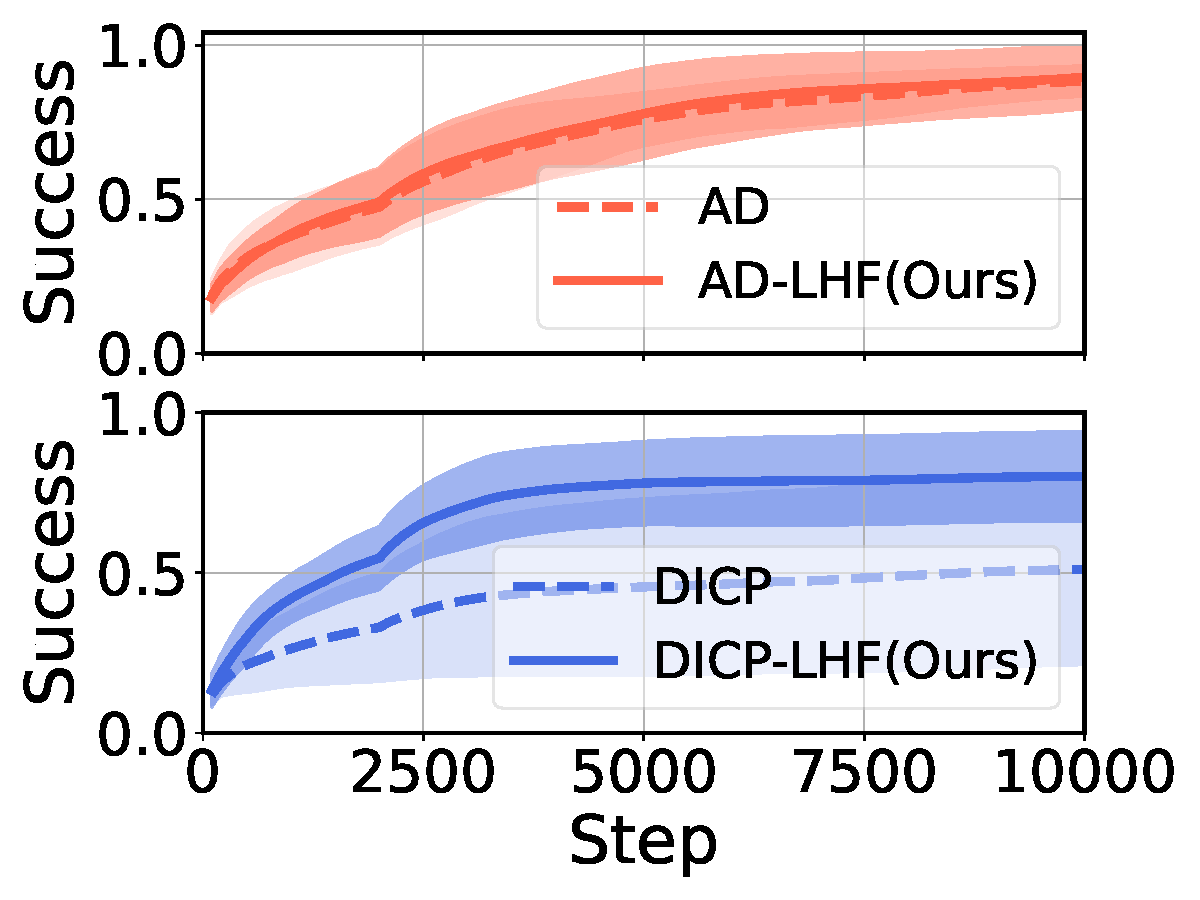
\includegraphics[width=1.0\columnwidth]{figures/reach-v2_AD_DICP_OUR_AD_OUR_DICP.pdf}
	\end{minipage}
}
\!\!\!\!\!\!\!
\subfigure[Reach-Wall]
{
	\begin{minipage}{0.25\linewidth}
	\centering 
	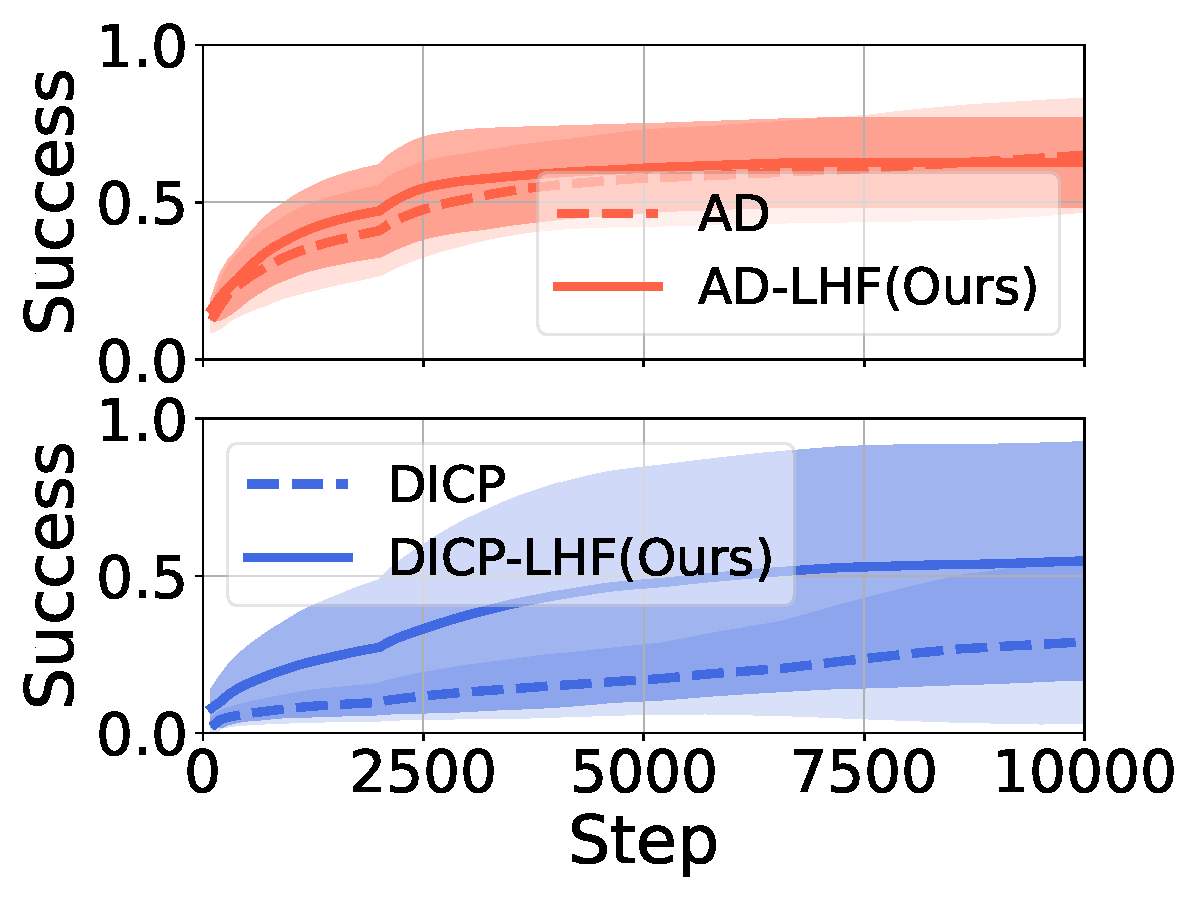
\includegraphics[width=1.0\columnwidth]{figures/reach-wall-v2_AD_DICP_OUR_AD_OUR_DICP.pdf}
	\end{minipage}
}
\!\!\!\!\!\!\!
\subfigure[Button-Press]
{
	\begin{minipage}{0.25\linewidth}
	\centering 
	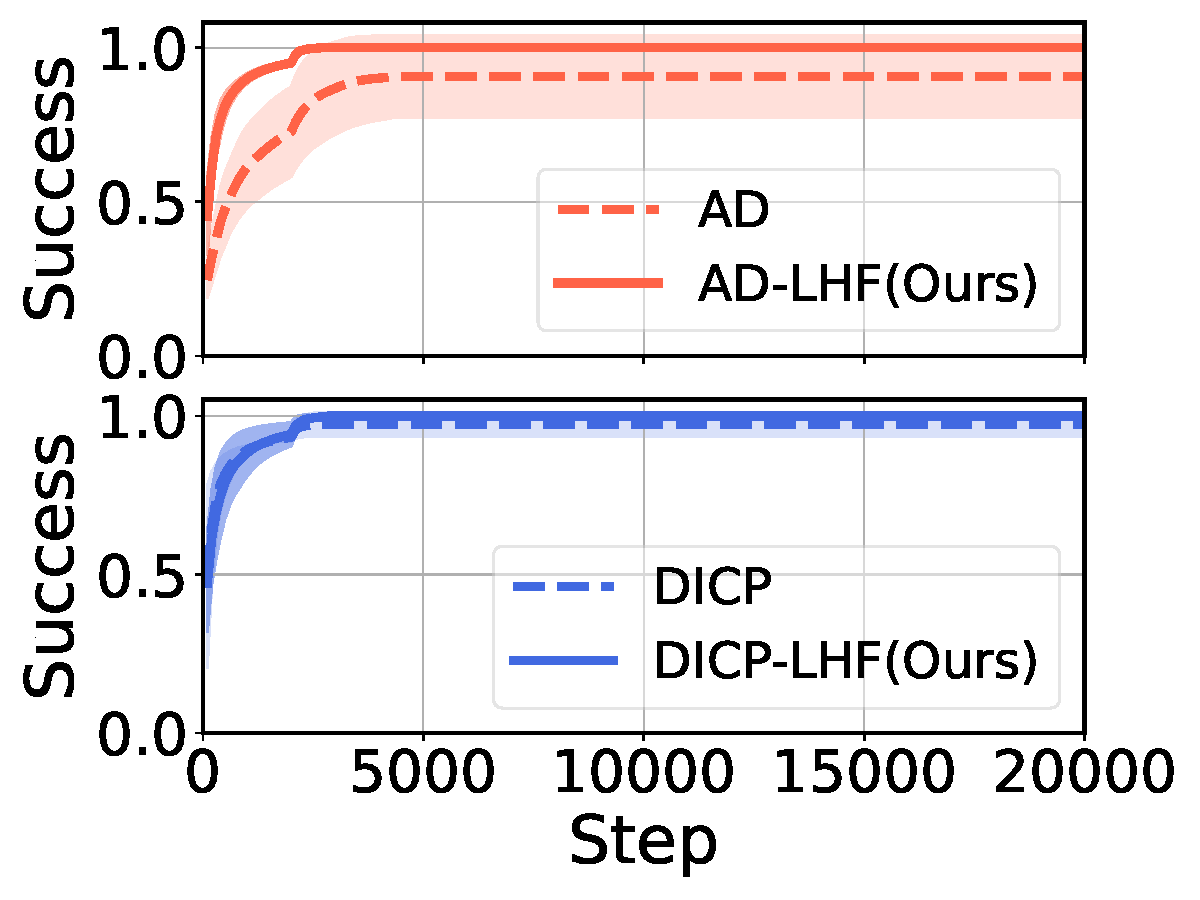
\includegraphics[width=1.0\columnwidth]{figures/button-press-v2_AD_DICP_OUR_AD_OUR_DICP.pdf}
	\end{minipage}
}
\!\!\!\!\!\!\!
\subfigure[Basketball]
{
	\begin{minipage}{0.25\linewidth}
	\centering 
	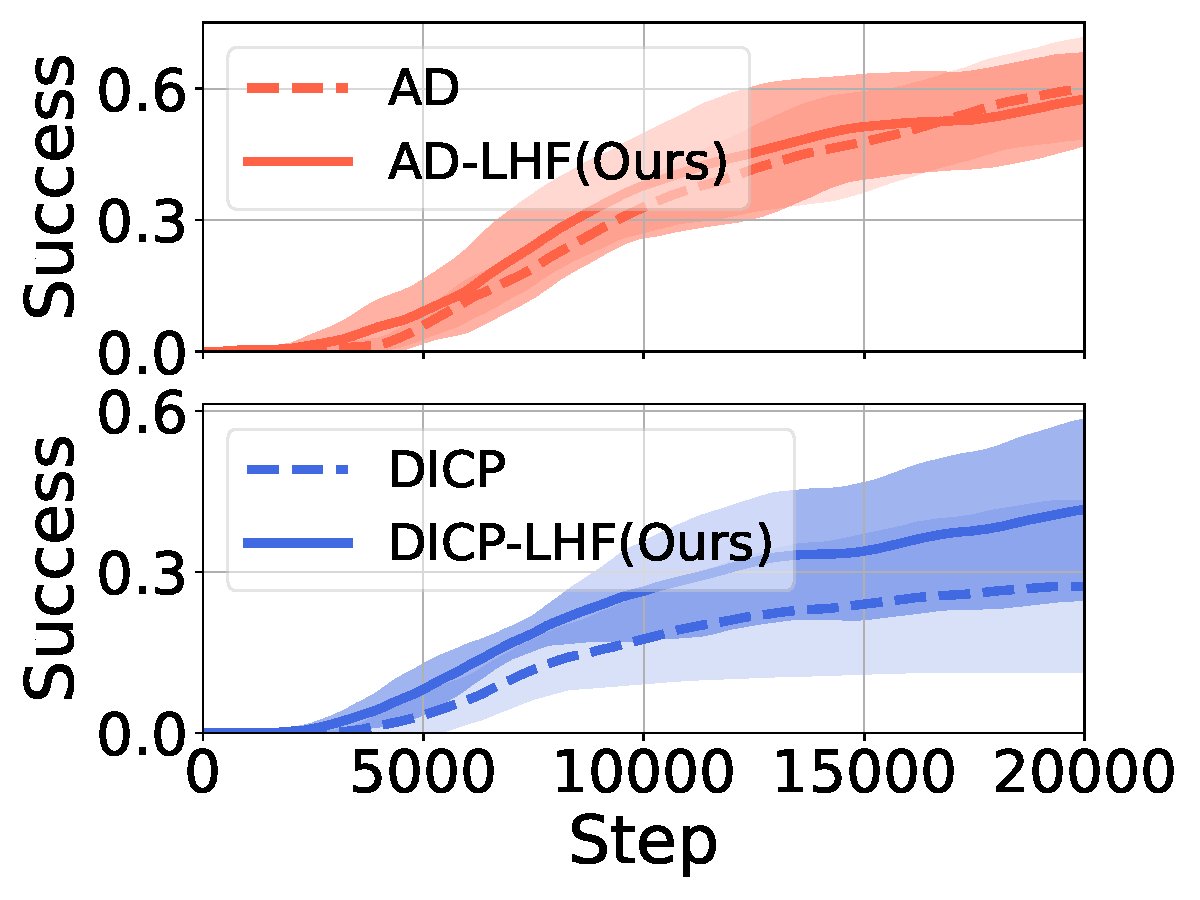
\includegraphics[width=1.0\columnwidth]{figures/basketball-v2_AD_DICP_OUR_AD_OUR_DICP.pdf}
	\end{minipage}
}
\\
\subfigure[Door-Unlock]
{
	\begin{minipage}{0.25\linewidth}
	\centering 
	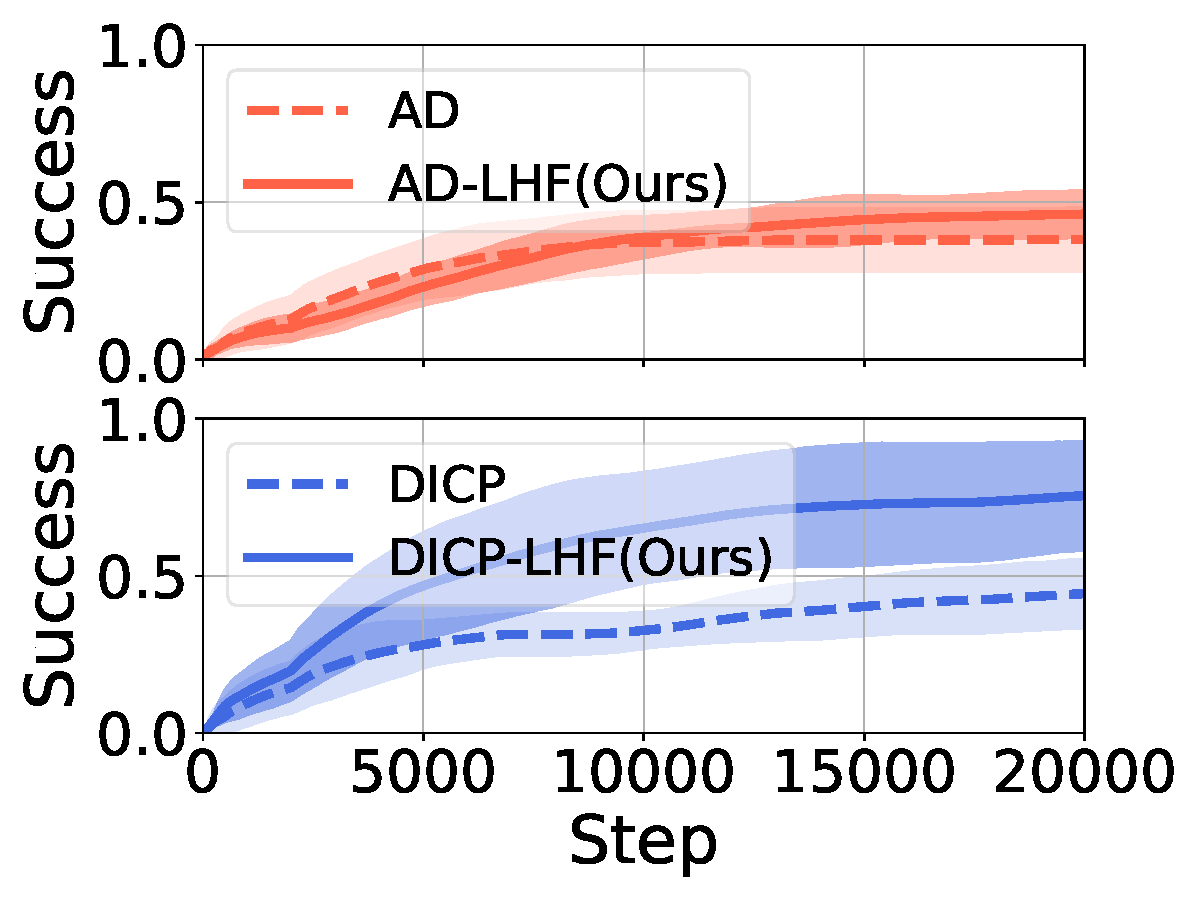
\includegraphics[width=1.0\columnwidth]{figures/door-unlock-v2_AD_DICP_OUR_AD_OUR_DICP.pdf}
	\end{minipage}
}
\!\!\!\!\!\!\!
\subfigure[Push]
{
	\begin{minipage}{0.25\linewidth}
	\centering 
	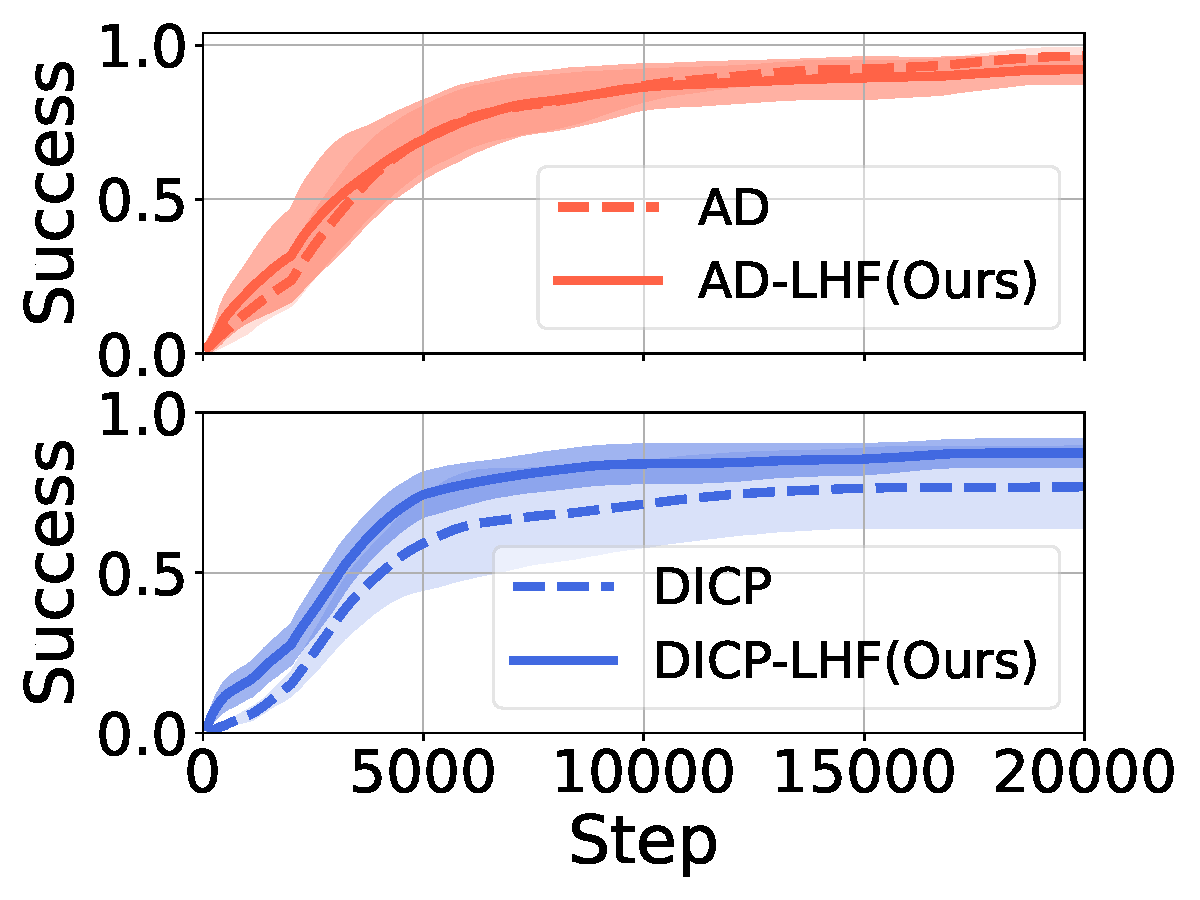
\includegraphics[width=1.0\columnwidth]{figures/push-v2_AD_DICP_OUR_AD_OUR_DICP.pdf}
	\end{minipage}
}
\!\!\!\!\!\!\!
\subfigure[Soccer]
{
	\begin{minipage}{0.25\linewidth}
	\centering 
	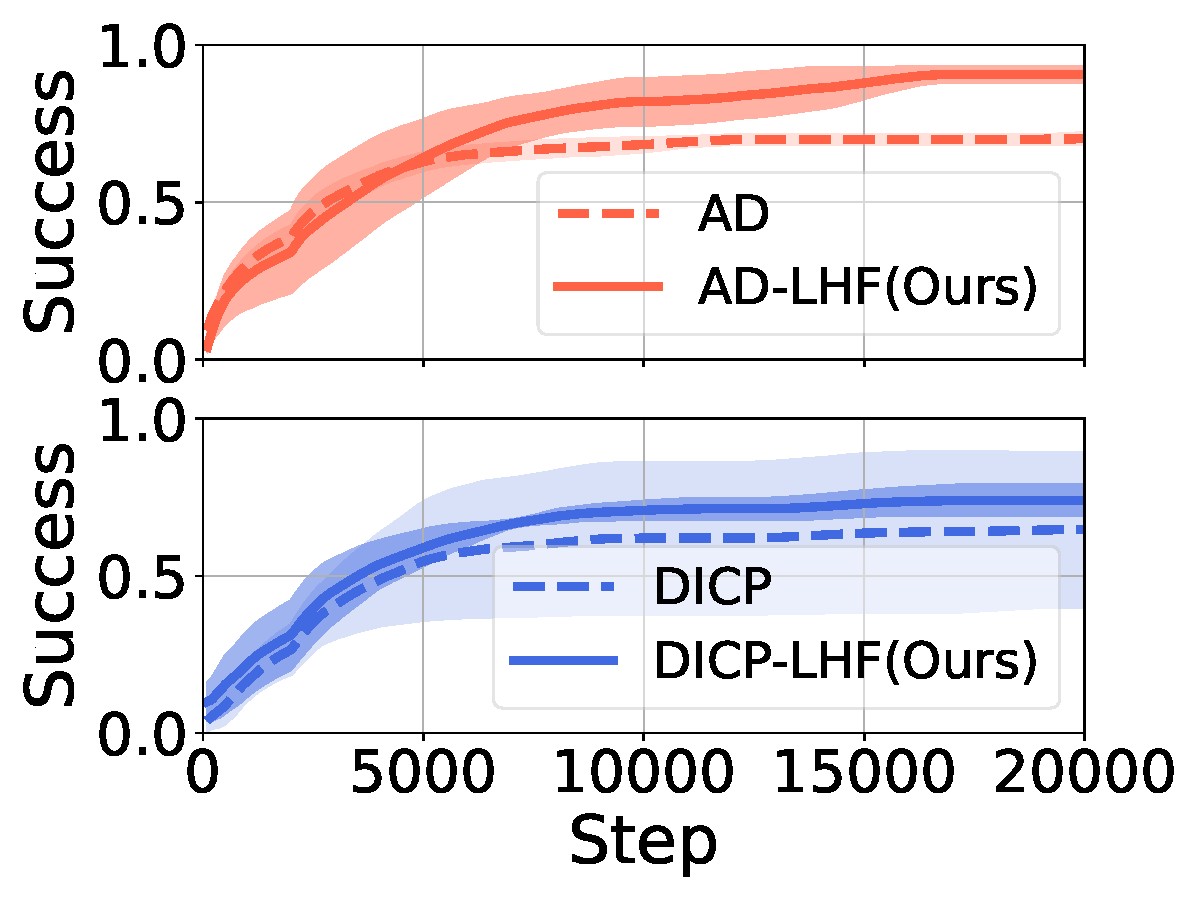
\includegraphics[width=1.0\columnwidth]{figures/soccer-v2_AD_DICP_OUR_AD_OUR_DICP.pdf}
	\end{minipage}
}
\!\!\!\!\!\!\!
\subfigure[Hand-Insert ]
{
	\begin{minipage}{0.25\linewidth}
	\centering 
	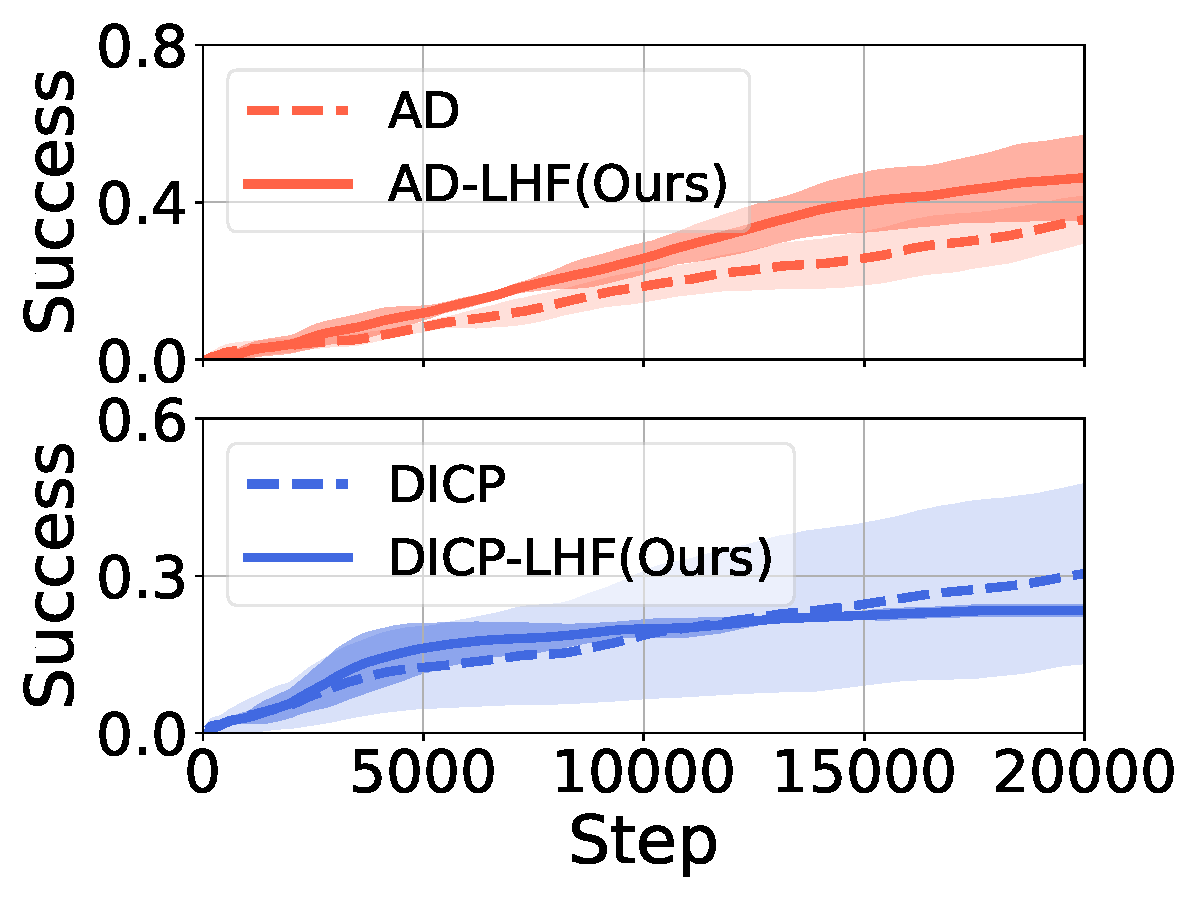
\includegraphics[width=1.0\columnwidth]{figures/hand-insert-v2_AD_DICP_OUR_AD_OUR_DICP.pdf}
	\end{minipage}
}
%
%
%
\caption{Learning curves of our LHF approach (solid lines) compared with original baselines (dashed lines) during the test. Each algorithm contains three independent runs with mean and std., provided with \textit{Meta-World-ML1} environments. The backbone algorithms include AD (red) and DICP (blue).}
\label{fig_metaworld_ppo}
\end{figure}
%%%%%%%%%%%%%%%%











\textbf{Can LHF enhance ICRL for complex continuous robotic tasks?}
%
Having verified the superior performance of our LHF approach using the four discrete environments (\textit{Darkroom}-type), we further evaluate LHF using more complicated continuous tasks of robotic manipulations: \textit{Meta-World-ML1}.
%
%
As mentioned earlier, we consider only AD and DICP as backbones, since DPT requires optimal action labels that are not available in \textit{Meta-World-ML1}.
%
%
The numerical results are presented in Figure~\ref{fig_metaworld_ppo} and Table~\ref{tab_metaworld_ppo}.
%
All positive relative enhancement in Table~\ref{tab_metaworld_ppo} except the cases of using AD in \textit{Push} and employing DICP in \textit{Hand-Insert} implies the consistently improved performance of LHF over the baselines across most backbone algorithms and \textit{Meta-World-ML1} tasks. 
%
On average, AD and DICP yield relative enhancements of $11.7\%$ and $46.2\%$, respectively. Notably, the certain scenario such as using DICP in \textit{Reach-Wall} can achieve more than $141\%$ performance enhancement.
























\subsection{Sensitivity Analysis}
\label{section_sensitivity}




In all experiments thus far, we have used a fixed stability coefficient ($\lambda = 1$) and a fixed linear sampling strategy to evaluate the general performance and robustness of LHF.
However, as shown in \eqref{eqn_metric}, $\lambda$ governs the trade-off between the improvement and stability, both of which are critical for ICRL pretraining. Therefore, it is essential to investigate how varying $\lambda$ influences the performance of LHF.
%
We evaluate the backbone algorithms AD and DICP on the \textit{Darkroom} problem under varying stability coefficients $\lambda \in \{0, 0.5, 1, 2, 1000\}$. The corresponding numerical results are presented in Figure~\ref{fig_sensitivity}(a) and \ref{fig_sensitivity}(b).
%
Notably, for both algorithms, the settings $\lambda \in \{0.5, 1, 2\}$ consistently outperform the two extremes $\lambda \in \{0, 1000\}$, highlighting the significance of balancing the improvement and stability during the ICRL pertaining. Overall, even the worst-case performance under varying $\lambda$ remains comparable to the original baseline without LHF, demonstrating the robustness of our approach.



%%%%%%%%%%%%%%%%
\begin{figure}[ht]
\centering 
\setcounter{subfigure}{0}
\subfigure[AD with varying $\lambda$]
{
	\begin{minipage}{0.25\linewidth}
	\centering 
    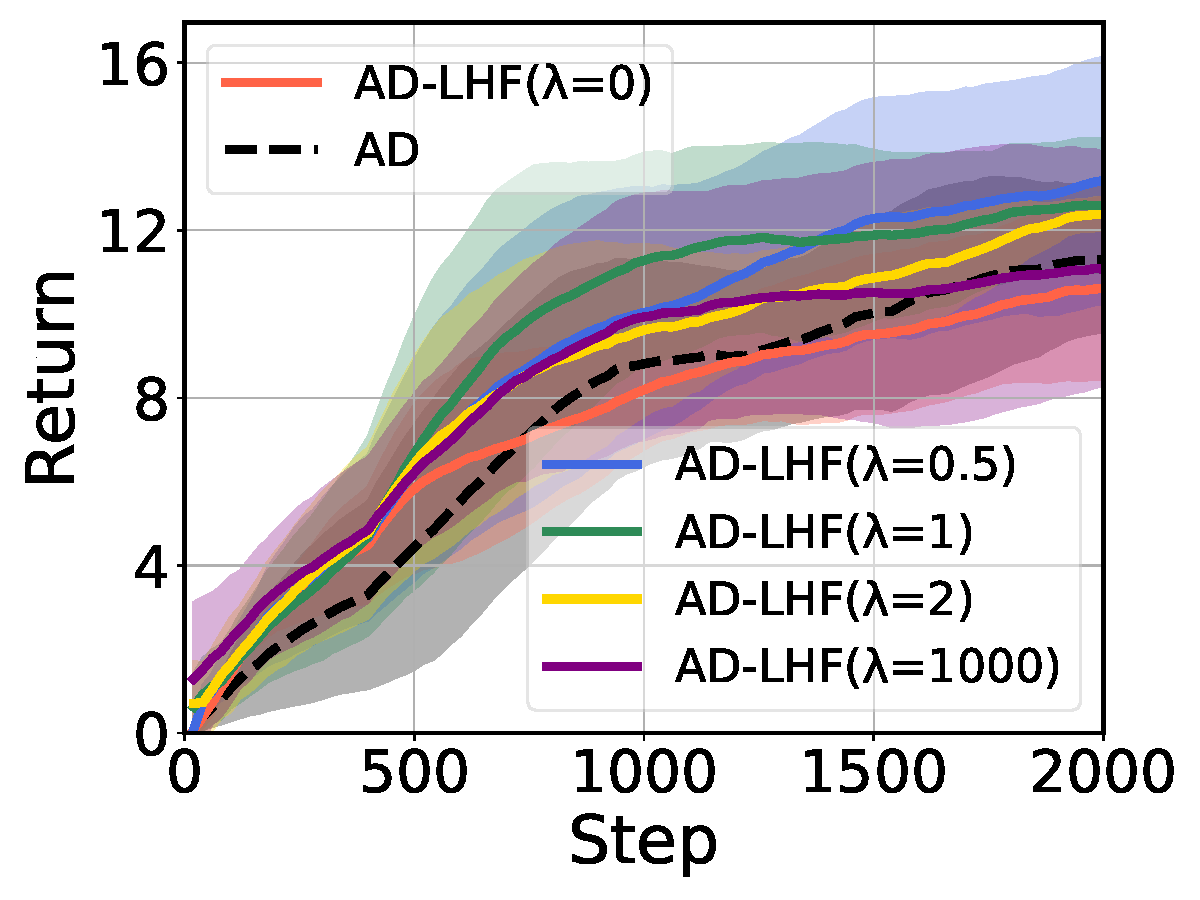
\includegraphics[width=1.0\columnwidth]{figures/Compare_AD_Various_dataset_linear.pdf}
	\end{minipage}
}
\!\!\!\!\!\!\!
\subfigure[DICP with varying $\lambda$]
{
	\begin{minipage}{0.25\linewidth}
	\centering 
	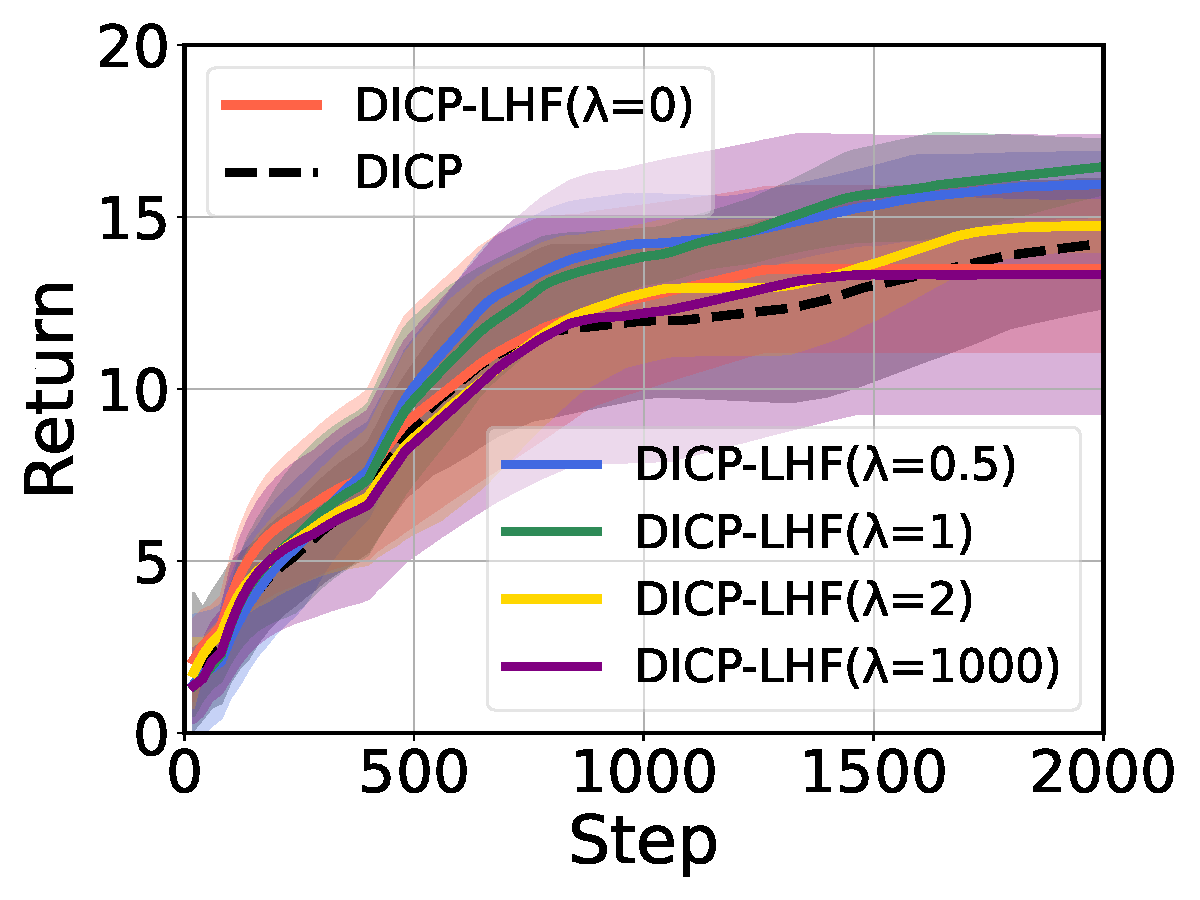
\includegraphics[width=1.0\columnwidth]{figures/Compare_DICP_Various_dataset_linear.pdf}
	\end{minipage}
}
\!\!\!\!\!\!\!
\subfigure[AD with varying $\alpha$]
{
	\begin{minipage}{0.25\linewidth}
	\centering 
	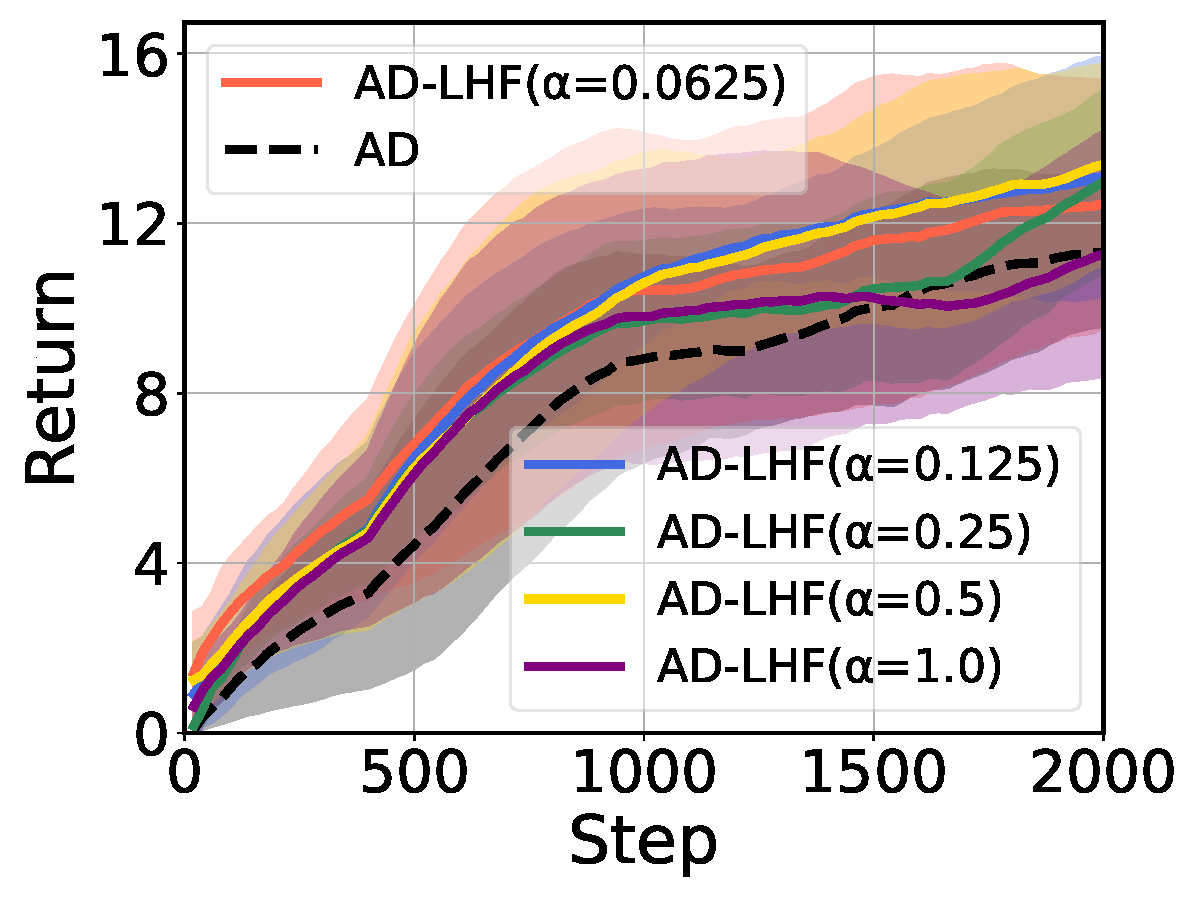
\includegraphics[width=1.0\columnwidth]{figures/Compare_AD_Various_dataset_softmax.pdf}
	\end{minipage}
}
\!\!\!\!\!\!\!
\subfigure[DICP with varying $\alpha$]
{
	\begin{minipage}{0.25\linewidth}
	\centering 
	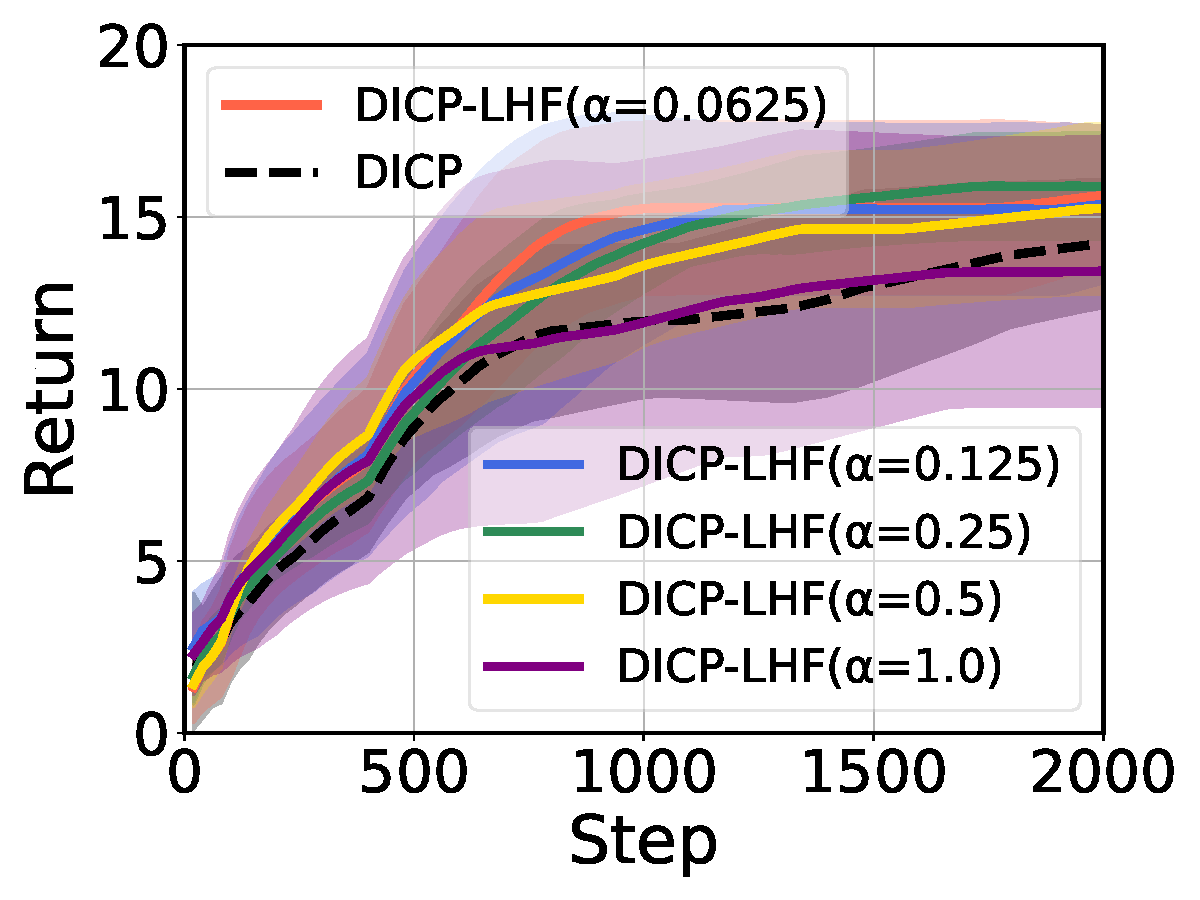
\includegraphics[width=1.0\columnwidth]{figures/Compare_DICP_Various_dataset_softmax.pdf}
	\end{minipage}
}
%
%
%
\caption{Learning curves of our LHF approach (solid lines) compared with original baselines (dashed lines) during the test. Each algorithm contains three independent runs with mean and std., provided with different stability coefficient $\lambda$ ((a) and (b)) and different temperature coefficient $\alpha$ in the Softmax sampling strategy ((c) and (d)). The backbone algorithms include AD and DICP.}
\label{fig_sensitivity}
\end{figure}
%%%%%%%%%%%%%%%%



Now we turn our attention to the sampling strategies. In this sensitivity analysis, we adopt a Softmax sampling strategy with a temperature coefficient $\alpha$ as follows 
%
\begin{align}\label{eqn_softmax_weight_func}
    \mathcal{P}_{\bar{w}}(U(\ccalD_i^l)) = \frac{U_\text{soft}(\ccalD_i^l) - \min_{l \in [N_l]} U_\text{soft}(\ccalD_i^l)}{\max_{l \in [N_l]} U_\text{soft}(\ccalD_i^l) - \min_{l \in [N_l]} U_\text{soft}(\ccalD_i^l)}, \, \text{where} \,\,  U_\text{soft}(\ccalD_i^l) = \frac{e^{U(\ccalD_i^l) / \alpha}}{\sum_l e^{U(\ccalD_i^l) / \alpha}}
\end{align}


We also implement AD and DICP on \textit{Darkroom} under varying temperature coefficients $\alpha \in \{0.0625, 0.125, 0.25, 0.5, 1\}$. The numerical results are presented in Figure~\ref{fig_sensitivity}(c) and \ref{fig_sensitivity}(d).
%
Both algorithms exhibit the superiority of LHF compared to the baselines, with even the worst-case results remaining comparable. This validates the robustness of LHF with respect to the sampling strategies.




Notice that all preceding experiments consider PPO as the source RL algorithm. To verify the algorithm-agnostic nature of LHF, we now employ SAC~\cite{haarnoja2018soft} to collect learning histories across four \textit{Meta-World-ML1} tasks: \textit{Reach}, \textit{Button-Press}, \textit{Push}, \textit{Soccer}. The details of SAC algorithm is provided in Appendix~\ref{append_collect_history}.
%
The numerical results are presented in Figure~\ref{fig_sac_source_rl} and Table~\ref{tab_sac_source_rl} in Appendix~\ref{append_addition_result_sensitivity_sourceRL}. 
%
% All positive enhancement in Table~\ref{tab_sac_source_rl} except for the case of using DICP in \textit{Soccer} implies the consistently improved performance of LHF over the baselines across most backbone algorithms and problems, provided with SAC dataset. 
%
On average, AD and DICP yield relative enhancement of $44.0\%$ and $9.2\%$, respectively. LHF in the certain scenario such as employing AD in \textit{Reach} achieves more than $110\%$ performance enhancement. These findings empirically validate the robustness of LHF with respect to the source RL algorithm.






















































\section{Discussion}
\label{discussion_section}
%
In this work, we introduce the learning history filtering (LHF), a simple yet effective dataset preprocessing approach to enhance ICRL by addressing the issue of inheriting source suboptimality in the dataset. LHF operates by reweighting and filtering the learning histories according to their inherent improvement and stability, offering a general plug-in mechanism compatible with existing ICRL algorithms.
%
Through a series of evaluations on \textit{Darkroom}-type problems and \textit{Meta-World-ML1} robotic manipulation tasks, we demonstrate the superior performance and robustness of LHF aross various scenarios. The performance enhancement is even more obvious on the noisy datasets, further underscoring the significance of filtering suboptimal histories.
%
Our findings also demonstrate the importance and success of data-centric interventions in advancing the performance of ICRL.




\textbf{Limitations and Future Work.}
%
Our LHF approach is inspired by the WERM schema, which is natural and intuitive from an optimization perspective. However, it remains an open and interesting direction in the future to theoretically characterize the filtering mechanism in the specific context of ICRL with respect to e.g., generalization error~\cite{lin2023transformers}.
%
Moreover, existing ICRL methods fall into the category of unconstrained RL, which remains inadequate for safety-critical applications. Future work could incorporate an extra cost function, analogous to reward, to enable the in-context safe RL.











%%%%%%%%%%%%%%%%%%%%%%%%%%%%%%%%%%%%%%%%%%%%%%%%%%%%%%%%%%%%

\clearpage


\section*{Acknowledgement}
%
The authors would like to thank Jaehyeon Son for the valuable discussions as well as the open-source implementations of DICP.



\bibliography{neurips_2025}
\bibliographystyle{unsrt}








%%%%%%%%%%%%%%%%%%%%%%%%%%%%%%%%%%%%%%%%%%%%%%%%%%%%%%%%%%%%
\clearpage


\appendix

\section{Implementation and Experiment Details}

% Appendix A.1: We collect learning histories

% Appendix A.2: We use three backbone ICRL algorithms to train

% Appendix A.3: All three backbone algorithms use Transformers. Introduce the transformer structure and corresponding hyperparameters


\subsection{Collecting Learning Histories}
\label{append_collect_history}

In this work, we employ the Stable Baselines 3 (SB3) implementations of Proximal Policy Optimization (PPO) \citep{schulman2017proximal} and Soft Actor–Critic (SAC) \citep{haarnoja2018soft} to generate learning histories for ICRL pre-training. PPO is an on-policy algorithm that stabilises updates with a clipped surrogate objective, whereas SAC is an off-policy, entropy-regularised actor–critic method that encourages exploration via a maximum-entropy objective. SB3 provides well-tested PyTorch versions of both algorithms under a uniform API, which facilitates reproducibility. 
%
Following DICP \cite{son2025distilling}, we summarize the key hyperparameters in Table \ref{tab:hyp-ppo-sac} while the remaining hyperparameters are kept at default.


\newcommand{\adjvcenter}[1]{%
  \raisebox{-.55\height}[0pt][0pt]{#1}%
}

\begin{table}[h]
\caption{Key hyperparameters for PPO and SAC.}
\label{tab:hyp-ppo-sac}
\scriptsize
\centering
\setlength{\tabcolsep}{3pt}
\begin{tabular}{l c c c c c c}
\toprule
\multirow{2}{*}{\adjvcenter{\textbf{Hyperparameter}}} &
\multicolumn{5}{c}{\textbf{PPO}} & \textbf{SAC}\\
\cmidrule(lr){2-6}\cmidrule(lr){7-7}
& \textit{Darkroom} & \textit{Darkroom-Permuted} &
  \textit{Darkroom-Large} & \textit{Dark Key-to-Door} &
  \textit{Meta-World-ML1} & \textit{Meta-World-ML1}\\
\midrule
batch size              & 50  & 50  & 50  & 100 & 200 & 128\\
discount factor         & 0.99& 0.99& 0.99& 0.99& 0.99& 0.99\\
source learning rate    & $3\times10^{-4}$ & $3\times10^{-4}$ &
                          $3\times10^{-4}$ & $3\times10^{-4}$ &
                          $3\times10^{-4}$ & $3\times10^{-4}$\\
\# of processes         & 8   & 8   & 8   & 8   & 8   & 8\\
\# of learning histories& 100 & 100 & 100 & 100 & 100 & 100\\
total transitions       & $1\times10^{5}$ & $1\times10^{5}$ & $1\times10^{5}$ &
                          $1\times10^{5}$ & $1\times10^{6}$ & $1\times10^{6}$\\
\bottomrule
\end{tabular}
\end{table}











\subsection{Backbone ICRL Algorithms}
\label{append_backboneICRLalgo}

\paragraph{Algorithm Distillation (AD).}
AD \citep{laskin2022context} is an in-context RL framework for transforming the training process of a source RL algorithm into a single in-context policy. Concretely, AD first collects learning histories from an RL algorithm deployed on a large substantial amount of tasks. Each learning history is a multi-episode record of transitions $\bigl(s_t^{(i)},\,a_t^{(i)},\,r_t^{(i)}\bigr)$, capturing how the source algorithm explores and improves its policy. A TM is then trained, via supervised learning, to predict the source algorithm’s action $a_t^{(i)}$ from the preceding history
\begin{equation}
\label{eq:ad}
\gL_{\mathrm{AD}}(\theta)
=
- \sum_{i \in [N]}\!
  \sum_{t \in [T]}
  \log
  M_{\theta}\!\Bigl(
      a_t^{(i)}
      \,\Bigm|\,
      \ccalC_{t-1}^{(i)},\,  
      s_t^{(i)}
  \Bigr),
\end{equation}
%
 where $\ccalC_{t-1}^{(i)}$ denotes the context of the $i$-th learning history up to step $t{-}1$, and $M_\theta(\cdot\mid\cdot)$ is the model’s predicted action distribution. Once trained, the TM can be deployed \emph{without} any parameter updates on new tasks, adapting online by conditioning on its own growing history. By imitating \emph{entire learning sequences} rather than a single policy snapshot, AD yields an in-context learner that inherits effective exploration and credit-assignment strategies from its source algorithm.


\paragraph{Decision Pretrained Transformer (DPT).}
DPT~\cite{lee2024supervised} is another in-context RL method that pre-trains a TM to predict optimal (or near-optimal) actions given a sampled query state and context during the ICRL pretraining. Throughout this paper, we consider the query state and context in DPT to be sampled from the learning histories, as introduced in the original DPT paper~\cite{lee2024supervised}.
In practice, DPT requires either an oracle or a well-trained expert policy that can generate high-quality actions for labeling all pretraining tasks.
Formally, the DPT objective can be written as
\begin{equation}
    \label{eq:dpt2}
    \gL_{\mathrm{DPT}}(\theta)
    \;=\;
- \sum_{i \in [N]}\!
  \sum_{t \in [T]}
      \log\,
      M_{\theta}\!\Bigl(
        a_t^{(i), \star}
        \;\Bigm|\;
        \ccalC_{t-1}^{(i)},\,  
         s_t^{(i)}
      \Bigr),
\end{equation}
where $a_t^{(i), \star}$ denotes the optimal action for the state $s_t^{(i)}$ in the underlying MDP. 
Under mild conditions on the task distribution and sufficient model capacity, DPT can approximate a Bayesian posterior over tasks, thus emulating posterior-sampling-style updates in context. Consequently, it is able to learn efficient strategies for online exploration and offline decision-making purely through a supervised objective.

\paragraph{Distillation for In-Context Planning (DICP).}  
%
DICP~\citep{son2025distilling} is a \emph{model-based} extension of ICRL, built on AD~\citep{laskin2022context} and DPT~\citep{lee2024supervised}. 
Instead of only predicting an action for each in-context step, DICP also learns a \emph{dynamics model} in-context, enabling the agent to simulate future transitions before acting.
Formally, a TM is pretrained to model not only $a_t$ (action), but also $(r_t,\,s_{t+1}, R_t)$ (reward, next state, return-to-go), yielding an objective as follows
% producing a likelihood of these outcomes given its contextual history $\ccalC_{t-1}^{(i)}$ and current action $a_t$:
\begin{equation}
\label{eq:dicp}
\begin{aligned}
\gL_{\mathrm{DICP}}(\theta)
= &~
\underbrace{
- \sum_{i \in [N]}\!
  \sum_{t \in [T]}
  \log 
  M_{\theta}\Bigl(
    a_{t}^{(i)}
    \,\Bigm|\,
    \ccalC_{t-1}^{(i)},\
    s_{t}^{(i)}
  \Bigr)
}_{\text{\normalsize imitation of the source algorithm}}
\\[0.3em]
& \quad
+ \;
\xi \;
\underbrace{
  \Big(- \sum_{i \in [N]}\!
  \sum_{t \in [T]}
  \log 
  W_{\theta}\Bigl(
    r_{t}^{(i)},\,s_{t+1}^{(i)},\, R_t^{(i)}
    \,\Bigm|\,\ccalC_{t-1}^{(i)},\,s_{t}^{(i)}, \,
    a_{t}^{(i)}
  \Bigr)\Big)
}_{\text{\normalsize modeling dynamics}}
\,,
\end{aligned}
\end{equation}
%
where \(\xi\) is a hyperparameter that balances algorithm imitation and dynamics modeling.
Once pretrained, at test time DICP applies \emph{planning} (e.g.\ beam or greedy search) over multiple simulated trajectories drawn from $W_{\theta}(\cdot)$ to choose an action that maximizes predicted rewards. By leveraging the learned dynamics model in-context, DICP enables the improvement of ICRL performance especially when the source algorithm exhibits suboptimal behaviors. Thus, compared to prior ICRL methods, DICP enables more deliberate decision-making through model-based search, further enhancing the sample efficiency and adaptability.



\subsection{Transformer Models}
\label{append_transformer_hyperparameter}

TMs employed in this work are based on the open-source \emph{TinyLlama} framework~\citep{zhang2024tinyllama}, 
a lightweight yet powerful model designed for efficient large language model variants. 
Our experiments cover four discrete tasks (\textit{Darkroom}, \textit{Darkroom-Permuted}, \textit{Darkroom-Large}, \textit{Dark Key-to-Door}), which we collectively refer to as ``Gridworld'', and one continuous robotic manipulation benchmark (\textit{Meta-World-ML1}), denoted as ``Metaworld''. 
Table~\ref{tab:hyp-tf} provides the specific hyperparameter configurations we consider for AD, DICP, and DPT in these respective settings.
%
\begin{table}[h]
\caption{Key hyperparameters for discrete tasks (\textit{Gridworld}) and continuous robotic manipulation tasks (\textit{Metaworld}).}
\label{tab:hyp-tf}
% \small
\centering
\begin{tabular}{lcc}
\toprule
\textbf{Hyperparameter} & \textbf{Gridworld (AD, DICP, DPT)} & \textbf{Metaworld (AD, DICP)} \\
\midrule
attention dropout \& dropout   & 0.1           & 0.1 \\
% dropout               & 0.1           & 0.1 \\
$\beta_1$             & 0.9           & 0.9 \\
$\beta_2$             & 0.99          & 0.99\\
intermediate size    & 128           & 128 \\
learning rate         & $1\times10^{-2}$ & $1\times10^{-2}$ \\
embedding dimension          & 32            & 32  \\
\# of heads           & 4             & 4   \\
\# of layers          & 4             & 4   \\
optimizer             & AdamW         & AdamW \\
scheduler             & cosine decay  & cosine decay \\
weight decay         & 0.01          & 0.01 \\
\bottomrule
\end{tabular}
\end{table}




\subsection{Complete Process of ICRL via Learning History Filtering (LHF)}
\label{append_complete_pseudocode}
Below we provide a pseudo-code description of the full procedure for
applying learning history filtering (LHF) to ICRL. In
Algorithm~\ref{alg_whole}, we first filter the collected learning histories (lines~2--17), producing a refined pretraining dataset $\ccalD_{\text{LHF}}$. We then follow the standard pretraining and test processes (lines~18--28).
%with the only difference being that data sampled for supervised training now comes from the filtered set $\ccalD_{\text{LHF}}$ instead of the original dataset.
\begin{algorithm}
\caption{In-Context Reinforcement Learning via Learning History Filtering}         
\label{alg_whole}
\begin{algorithmic}[1]

        \STATE \textbf{Require:} Pretraining dataset $\{\ccalD_i^l\}$ with $i \in [N_i], l \in [N_l]$, empty LHF dataset $\ccalD_\text{LHF}$, initial model parameters $\theta$, test environment distribution $\ccalT_{\text{test}}$, number of test episodes $N_E$

        \STATE \green{\textbf{// Dataset Preprocessing}}
        %%%%%%%%%%%%%%%%%%%%%%%%%%%%%%%%%%%%%%%%%%%%%%%%
        \FOR{$i$ in $[N_i]$}

            \STATE Let $\ccalD_i' = \emptyset$
            \WHILE{$|\ccalD_i'| < |\ccalD_i|$}
                    
                \FOR{$l$ in $[N_l]$}

                    \STATE Compute the unified metric $U(\ccalD_i^l)$ by \eqref{eqn_metric}
                    \STATE Compute the weighted probability $\mathcal{P}_{\bar{w}}(U(\ccalD_i^l))$ for the learning history $\ccalD_i^l$ by \eqref{eqn_linear_weight_func}
            
                    \STATE Sample a uniform random variable $v \sim \ccalU[0, 1]$

                    \STATE Add the learning history $\ccalD_i^l$ to $\ccalD_i'$ \textbf{if} $v \leq \mathcal{P}_{\bar{w}}(U(\ccalD_i^l))$
                    
                    \IF{$|\ccalD_i'| = |\ccalD_i|$}
                    \STATE break
                    \ENDIF
                \ENDFOR
            \ENDWHILE
 
            \STATE $\ccalD_\text{LHF} \leftarrow \ccalD_\text{LHF} \cup \ccalD_i'$
        \ENDFOR

        
        \STATE \green{\textbf{// Pretraining}}
        %%%%%%%%%%%%%%%%%%%%%%%%%%%%%%%%%%%%%%%%%%%%%%%%
        \WHILE{not converged}
            \STATE Sample $(\ccalC, s_q, a_l)$ from the LHF dataset $\ccalD_\text{LHF}$ and predict actions by $M_\theta(\cdot  | \ccalC, s_q)$
            \STATE Compute the loss in \eqref{eqn_icrl_obj_weighted_data} with respect to the action label $a_l$ and backpropagate to update $\theta$.
        \ENDWHILE

        
        \STATE \green{\textbf{// Test}}
        %%%%%%%%%%%%%%%%%%%%%%%%%%%%%%%%%%%%%%%%%%%%%%%%
        \STATE Sample unseen test environments $\tau \sim \ccalT_{\text{test}}$ and initialize empty context $\ccalC = \{\}$

        \FOR{$n$ in $[N_E]$}
                \STATE Deploy $M_\theta$ by sampling $a_t \sim M_{\theta}(\cdot  \mid \ccalC, s_t)$ at time step $t$
                \STATE Add $(s_0, a_0, r_0, \ldots)$ to $\ccalC$
        \ENDFOR
\end{algorithmic}
\end{algorithm}





\subsection{Environmental Setup}
\label{append_env_setup}



\paragraph{\textit{Darkroom}.}
%
\textit{Darkroom} is a two-dimensional navigation task with discrete state and action spaces. The room consists of $9 \times 9$ grids, with the agent reset in the middle of the room and an unknown goal randomly placed at any of these grids. The agent can select $5$ actions: go up, go down, go left, go right, or stay. The horizon length of \textit{Darkroom} is $20$. One challenge of this task arises from its sparse reward structure, i.e., the agent receives a reward of $1$ solely upon reaching the goal, and $0$ otherwise. 
%
Given $9 \times 9 = 81$ available goals, we randomly select $73$ of these goals ($\sim 90\%$) for pretraining and reserve the remaining $8$ goals ($\sim 10\%$ and unseen during pretraining) for test.


\paragraph{\textit{Darkroom-Permuted}.}
%
\textit{Darkroom-Permuted} is a variant of \textit{Darkroom} with the same state space and reward structure, with the agent reset in a fixed corner of the room and the goal placed in the opposite corner. In this problem, the action space undergoes a random permutation, yielding $5! = 120$ distinct tasks with each defined by a unique permutation of the action space. The horizon length of \textit{Darkroom-Permuted} is $50$. We randomly select $108$ tasks ($90\%$) for pretraining and reserve the remaining $12$ tasks ($10\%$ and unseen during pretraining) for test.



\paragraph{\textit{Darkroom-Large}.}
%
\textit{Darkroom-Large} adopts the same setup as in \textit{Darkroom}, yet with an expanded state space of $15 \times 15$ and a longer horizon of $50$. Thus, the agent must explore the room more thoroughly due to the sparse reward setting, rendering this task more challenging than \textit{Darkroom}. We still consider $90\%$ of $15 \times 15 = 225$ available goals for pretraining and the remaining unseen $10\%$ goals for test.


\paragraph{\textit{Dark Key-to-Door}.}
%
\textit{Dark Key-to-Door} also adopts the same setup as in \textit{Darkroom}, yet with an extra ``key'' positioned in any of  the grids. The agent must locate the key before reaching the door (goal). In this setting, it receives a one-time reward of $1$ upon finding the key, followed by an additional one-time reward of $1$ upon reaching the door, yielding a maximum return of $2$ within this environment.
%
Given $81 \times 81 = 6561$ available tasks by distinct positions of the key and door, we randomly select $6233$ tasks ($\sim 95\%$) for pretraining and reserve the remaining $328$ tasks ($\sim 5\%$) for test.



\paragraph{\textit{Meta-World-ML1}.}
%
\textit{Meta-World ML1}~\cite{yu2020meta} focuses on a single robotic manipulation task at a time, with $50$ predefined seeds each for the pretraining and test. These seeds correspond to different initializations of the object, goal, and agent. The agent is trained with varying goal configurations, and tested on new (unseen) goals. 
%
In this work, we focus on $8$ distinct tasks: \textit{Reach, Reach-Wall, Button-Press, Basketball, Door-Unlock, Push, Soccer, Hand-Insert}, each with a horizon of $100$ steps.













\section{Additional Experimental Results}



\subsection{ICRL with partial learning histories}
\label{append_addition_result_half_learn_hist}

Section~\ref{exp_numerical_result} presents the challenging scenario in which only the first \(50\%\) of each PPO learning history is retained.  
Discarding the last half of each learning history diminishes the improvement signal and shortens the credit-assignment horizon, yet LHF still surpasses the unfiltered baselines in nearly every algorithm–task combination. 
% AD records gains on all four tasks, yielding an average relative uplift of \(11.2\%\) and peaking at \(22.3\%\) on \textit{Darkroom–Large}.  DICP also benefits with a mean enhancement of \(4.9\%\) and the maximal enhancement exists in \textit{Darkroom}. DPT remains stable: three tasks exhibit positive gains, and the sole decline of \mbox{$-2.8\%$} on \textit{Darkroom--Permuted}—well within one standard deviation of the baseline—does not alter this conclusion. 
Complete results are reported in
Table~\ref{tab_darkrooms_half_learn_hist}, and the associated learning curves are depicted in Figure~\ref{fig_darkrooms_half_learn_hist}.


\begin{table}[ht]
    \caption{Relative enhancement (\%) of our LHF approach over the baselines, provided with half learning histories. Backbone algorithms: AD, DICP, DPT.}
    \label{tab_darkrooms_half_learn_hist}
    \centering
    \begin{tabular}{ccccc}
    \toprule
    Task & AD & DICP & DPT \\
    \midrule
     \textit{DarkRoom} & 14.1 & 11.4 & \textbf{19.6} \\
     \textit{Darkroom-Permuted} & \textbf{7.9} & 6.3 & -2.8 \\
     \textit{Darkroom-Large} & \textbf{22.3} & 0.9 & 16.4 \\
     \textit{Dark Key-to-Door} & 0.3 & \textbf{1.0} & 0.1 \\
    \midrule
    Average & \textbf{11.2} & 4.9 & 8.3 \\
    \bottomrule
    \end{tabular}
\end{table}




%%%%%%%%%%%%%%%%
\begin{figure}[ht]
\centering 
\setcounter{subfigure}{0}
\subfigure[Darkroom]
{
	\begin{minipage}{0.25\linewidth}
	\centering 
	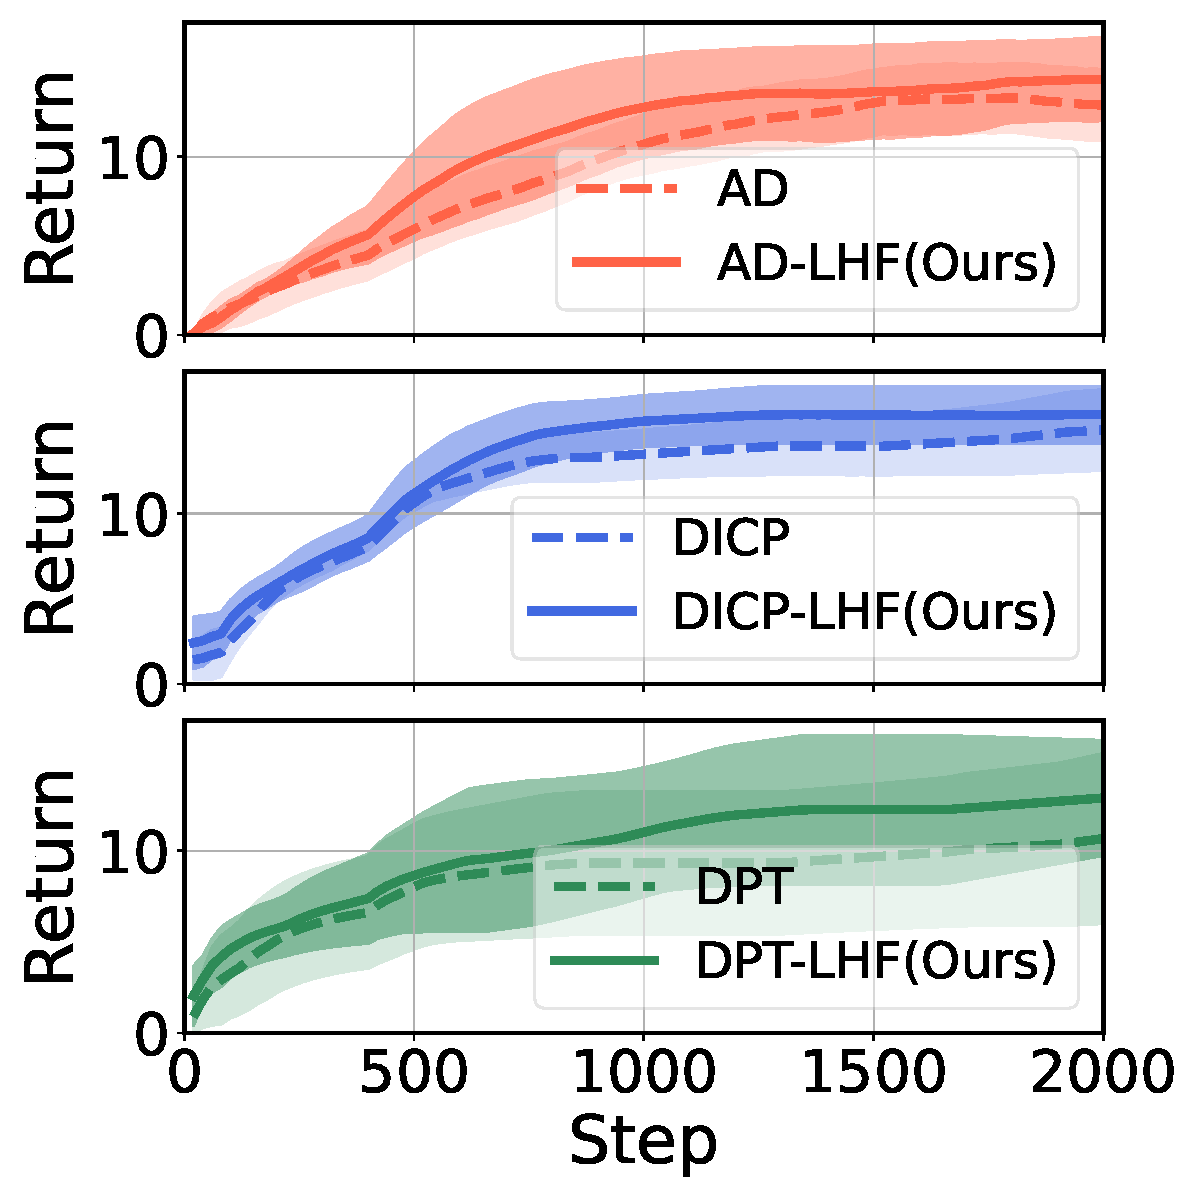
\includegraphics[width=1.0\columnwidth]{figures/HL_DR_AD_DICP_OUR_AD_OUR_DICP.pdf}
	\end{minipage}
}
\!\!\!\!\!\!\!
\subfigure[Darkroom-Permuted]
{
	\begin{minipage}{0.25\linewidth}
	\centering 
	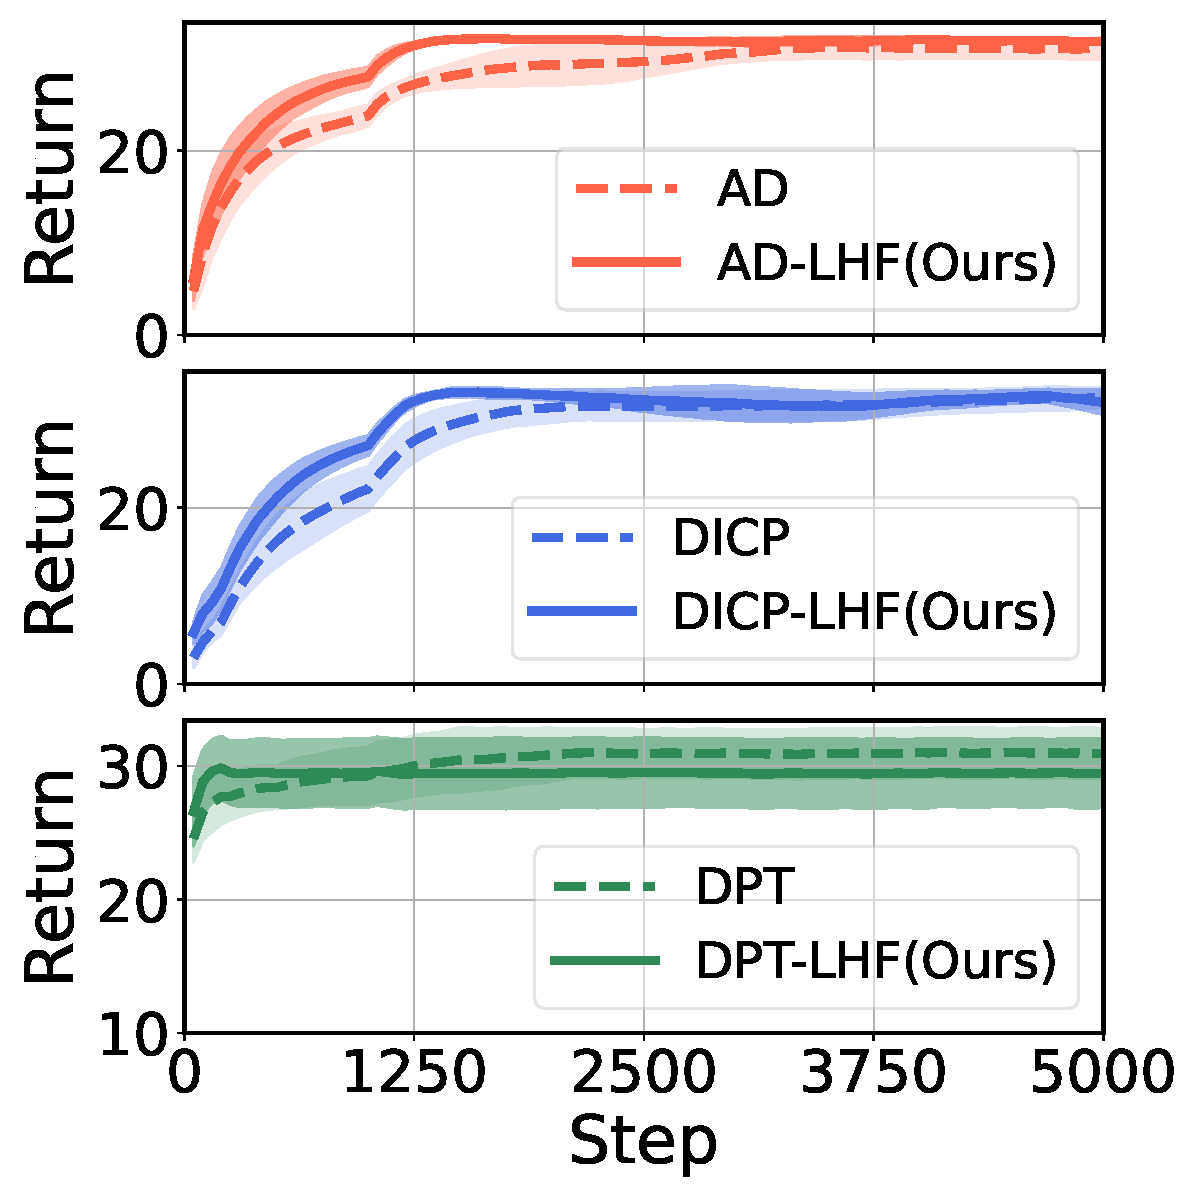
\includegraphics[width=1.0\columnwidth]{figures/HL_dr_permuted_AD_DICP_OUR_AD_OUR_DICP.pdf}
	\end{minipage}
}
\!\!\!\!\!\!\!
\subfigure[Darkroom-Large]
{
	\begin{minipage}{0.25\linewidth}
	\centering 
	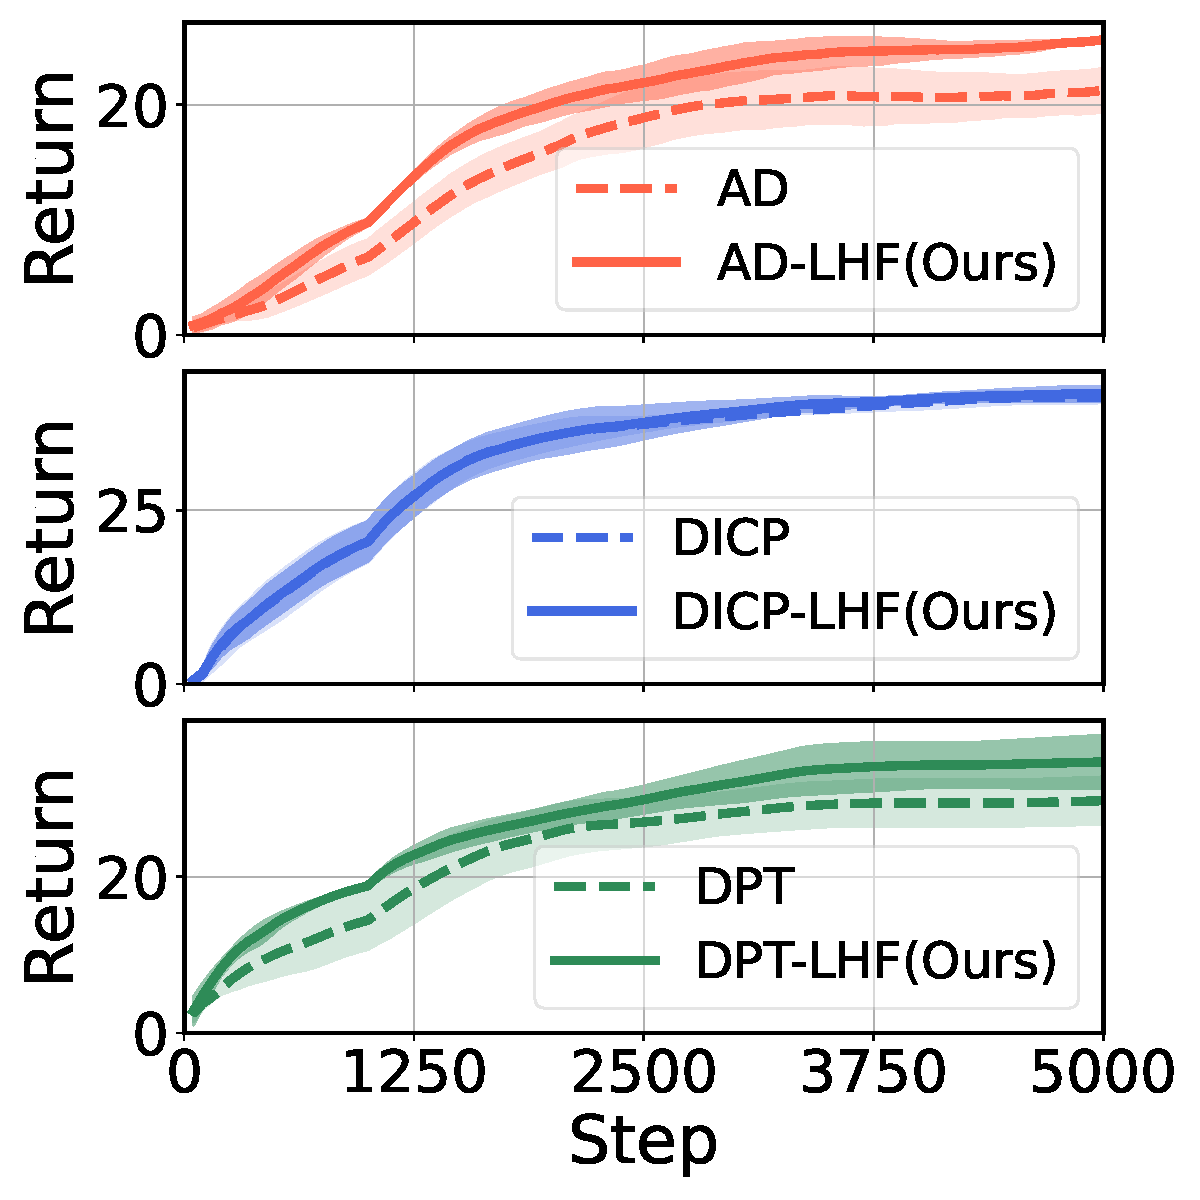
\includegraphics[width=1.0\columnwidth]{figures/HL_LDR_AD_DICP_OUR_AD_OUR_DICP.pdf}
	\end{minipage}
}
\!\!\!\!\!\!\!
\subfigure[Dark Key-to-Door]
{
	\begin{minipage}{0.25\linewidth}
	\centering 
	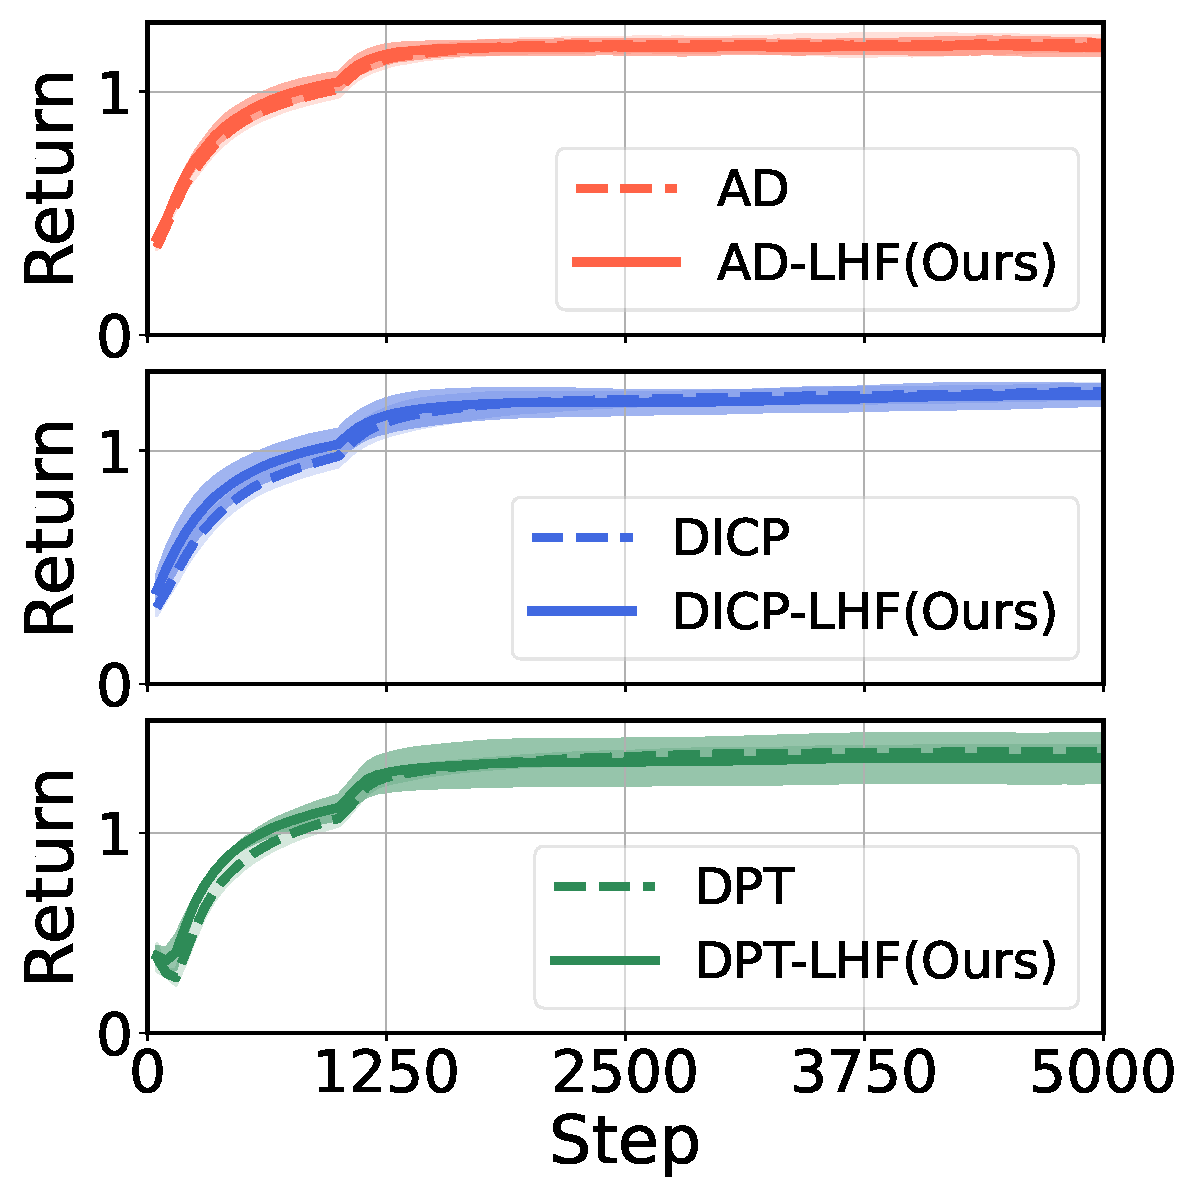
\includegraphics[width=1.0\columnwidth]{figures/HL_DKTD_AD_DICP_OUR_AD_OUR_DICP.pdf}
	\end{minipage}
}
%
%
%
\caption{Learning curves of our LHF approach (solid lines) compared with original baselines (dashed lines) during the test. Each algorithm contains three independent runs with mean and standard deviation, provided with half learning histories. The backbone algorithms include AD (red), DICP (blue), and DPT (green).}
\label{fig_darkrooms_half_learn_hist}
\end{figure}
%%%%%%%%%%%%%%%%











\subsection{ICRL with lightweight models}
\label{append_addition_result_lightweight_model}

Section~\ref{exp_numerical_result} also discusses the results of our LHF approach combined with a lightweight transformer model, which still demonstrates the superiority of LHF under the restricted model capacity. The detailed numerical results are referred to Table~\ref{tab_darkrooms_lightweight_model} and
Figure~\ref{fig_darkrooms_lightweight_model}.




% Comparing AD, DICP, and DPT with this lightweight architecture reveals
% the following. First, AD shows consistent improvement across all tasks,
% achieving a 12.6\% average relative boost and peaking at 22.4\% in
% \textit{Darkroom}. Similarly, DICP yields a mean improvement of 13.0\%
% and exhibits a 28.8\% jump in \textit{Darkroom}, suggesting that
% model-based planning especially benefits from filtering out suboptimal
% trajectories. By contrast, DPT’s performance is less sensitive overall,
% yet it still realizes gains on three of the four tasks despite a modest
% decline (-1.3\%) in \textit{Darkroom-Permuted}. In sum, these results
% confirm that LHF helps to mitigate low-quality data and strengthen
% in-context learning, even with a halved Transformer capacity.




\begin{table}[ht]
    \caption{Relative enhancement (\%) of our LHF approach over the baselines, provided with lightweight models. Backbone algorithms: AD, DICP, DPT.}
    \label{tab_darkrooms_lightweight_model}
    \centering
    \begin{tabular}{ccccc}
    \toprule
    Task & AD & DICP & DPT \\
    \midrule
     \textit{DarkRoom} & 22.4 & \textbf{28.8} & 10.6 \\
     \textit{Darkroom-Permuted} & \textbf{6.3} & 2.5 & -1.3 \\
     \textit{Darkroom-Large} & 4.9 & 2.1 & \textbf{5.4} \\
     \textit{Dark Key-to-Door} & 16.7 & \textbf{18.7} & 2.1 \\
    \midrule
    Average & 12.6 & \textbf{13.0} & 4.2 \\
    \bottomrule
    \end{tabular}
\end{table}






%%%%%%%%%%%%%%%%
\begin{figure}[ht]
\centering 
\setcounter{subfigure}{0}
\subfigure[Darkroom]
{
	\begin{minipage}{0.25\linewidth}
	\centering 
	\includegraphics[width=1.0\columnwidth]{figures/ReduceModel_darkroom_AD_DICP_OUR_AD_OUR_DICP.pdf}
	\end{minipage}
}
\!\!\!\!\!\!\!
\subfigure[Darkroom-Permuted]
{
	\begin{minipage}{0.25\linewidth}
	\centering 
	\includegraphics[width=1.0\columnwidth]{figures/Reduced_darkroom_Permuted_AD_DICP_OUR_AD_OUR_DICP.pdf}
	\end{minipage}
}
\!\!\!\!\!\!\!
\subfigure[Darkroom-Large]
{
	\begin{minipage}{0.25\linewidth}
	\centering 
	\includegraphics[width=1.0\columnwidth]{figures/Reduced_Model_Large_darkroom_AD_DICP_OUR_AD_OUR_DICP.pdf}
	\end{minipage}
}
\!\!\!\!\!\!\!
\subfigure[Dark Key-to-Door]
{
	\begin{minipage}{0.25\linewidth}
	\centering 
	\includegraphics[width=1.0\columnwidth]{figures/Reduced_darkkeytodoor_AD_DICP_OUR_AD_OUR_DICP.pdf}
	\end{minipage}
}
%
%
%
\caption{Learning curves of our LHF approach (solid lines) compared with original baselines (dashed lines) during the test. Each algorithm contains three independent runs with mean and standard deviation, provided with lightweight models. The backbone algorithms include AD (red), DICP (blue), and DPT (green).}
\label{fig_darkrooms_lightweight_model}
\end{figure}
%%%%%%%%%%%%%%%%









\subsection{Sensitivity analysis with respect to source RL algorithm}
\label{append_addition_result_sensitivity_sourceRL} 

Section~\ref{section_sensitivity} validates the robustness of our LHF performance in terms of the varying stability coefficient $\lambda$, distinct sampling strategies, and different source RL algorithms.
%
We present the numerical results of the first two in the main texts and exhibit the last one in Table~\ref{tab_sac_source_rl} and Figure~\ref{fig_sac_source_rl}.



% As shown in Figure~\ref{fig_sac_source_rl}, LHF consistently improves
% in-context learning under both AD and DICP. Even though SAC’s off-policy
% exploration pattern differs significantly from PPO’s on-policy updates,
% filtering still eliminates low-quality trajectories in ways that
% bolster final test performance. In particular, we observe dramatic
% uplifts for AD on \textit{Reach} (over 110\% improvement) and
% \textit{Push} (33.5\%). DICP gains more moderately but remains stable
% across tasks, occasionally dropping in certain edge cases (e.g. \textit{Soccer}
% in Table~\ref{tab_sac_source_rl}). Overall, these results confirm that
% the advantages of LHF do not hinge on which RL algorithm produced the
% offline dataset.



\begin{table}[ht]
    \caption{Relative enhancement (\%) of our LHF approach over the baselines, provided with datasets collected by SAC. Backbone algorithms: AD and DICP.}
    \label{tab_sac_source_rl}
    \centering
    \begin{tabular}{cccc}
    \toprule
    Task & AD & DICP \\
    \midrule
     \textit{Reach} & \textbf{110.4} & 10.7 \\
     \textit{Button-Press} & 8.6 & \textbf{26.8} \\
     \textit{Push} & \textbf{33.5} & 0.0 \\
     \textit{Soccer} & \textbf{23.3} & -0.6 \\
     \midrule
     Average & \textbf{44.0} & 9.2 \\
    \bottomrule
    \end{tabular}
\end{table}





%%%%%%%%%%%%%%%%
\begin{figure}[ht]
\centering 
\setcounter{subfigure}{0}
\subfigure[Reach]
{
	\begin{minipage}{0.25\linewidth}
	\centering 
	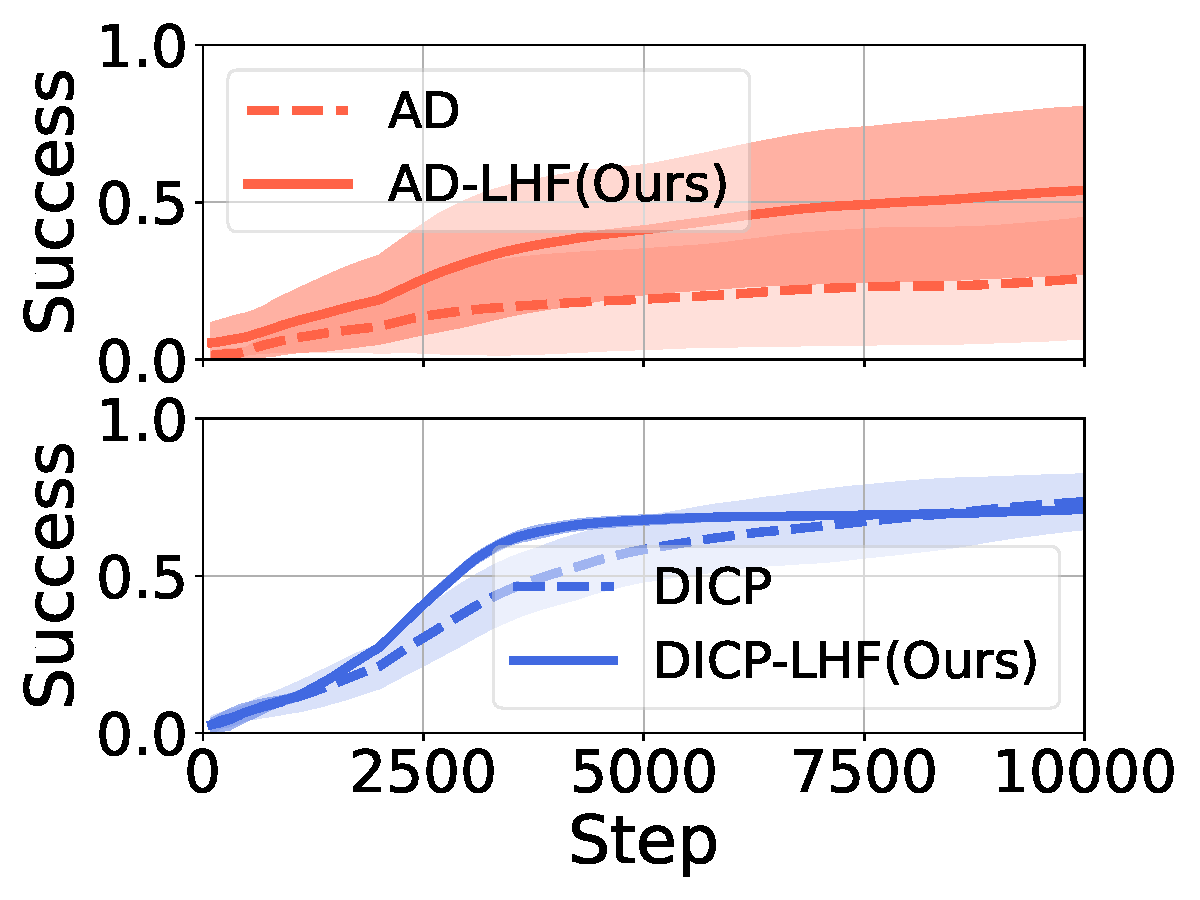
\includegraphics[width=1.0\columnwidth]{figures/reach-v2_SAC.pdf}
	\end{minipage}
}
\!\!\!\!\!\!\!
\subfigure[Button-Press]
{
	\begin{minipage}{0.25\linewidth}
	\centering 
	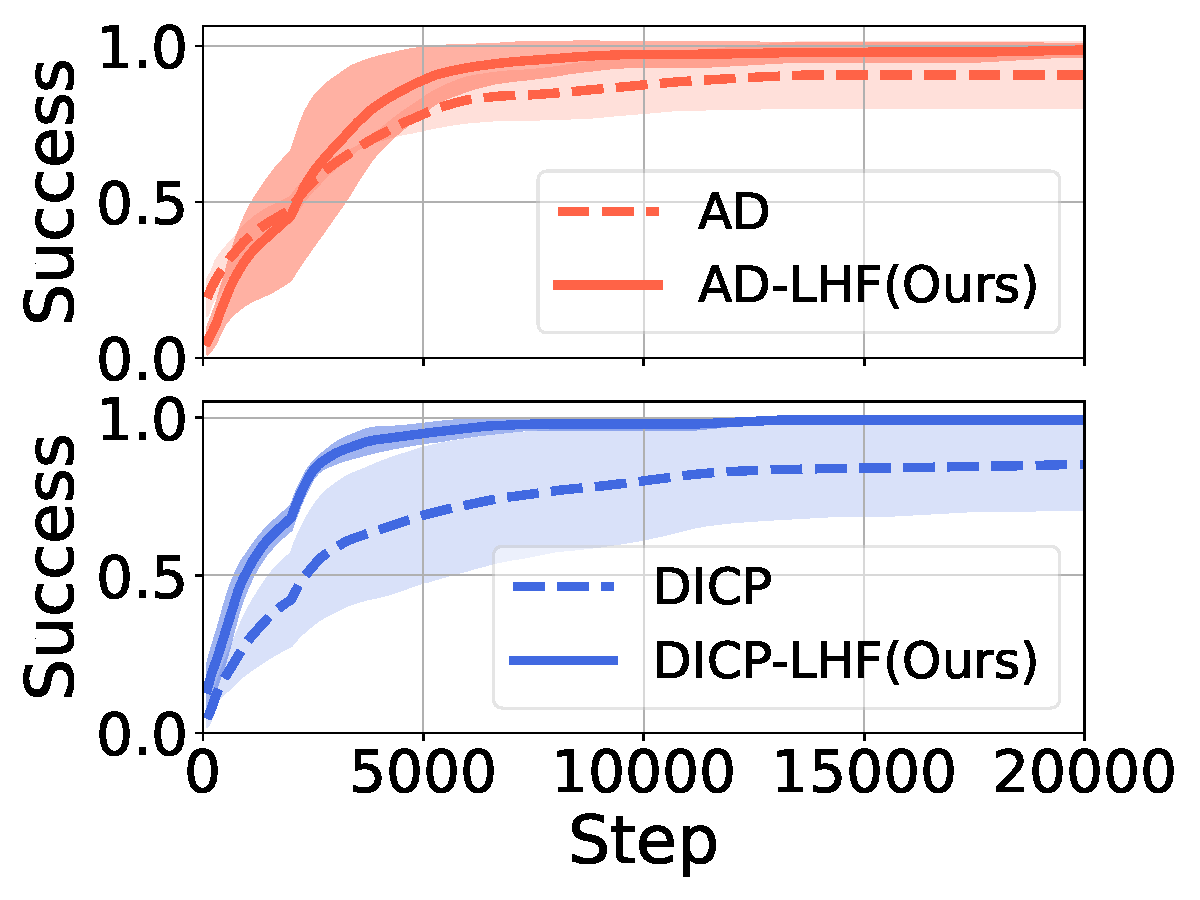
\includegraphics[width=1.0\columnwidth]{figures/button-press-v2_SAC.pdf}
	\end{minipage}
}
\!\!\!\!\!\!\!
\subfigure[Push]
{
	\begin{minipage}{0.25\linewidth}
	\centering 
	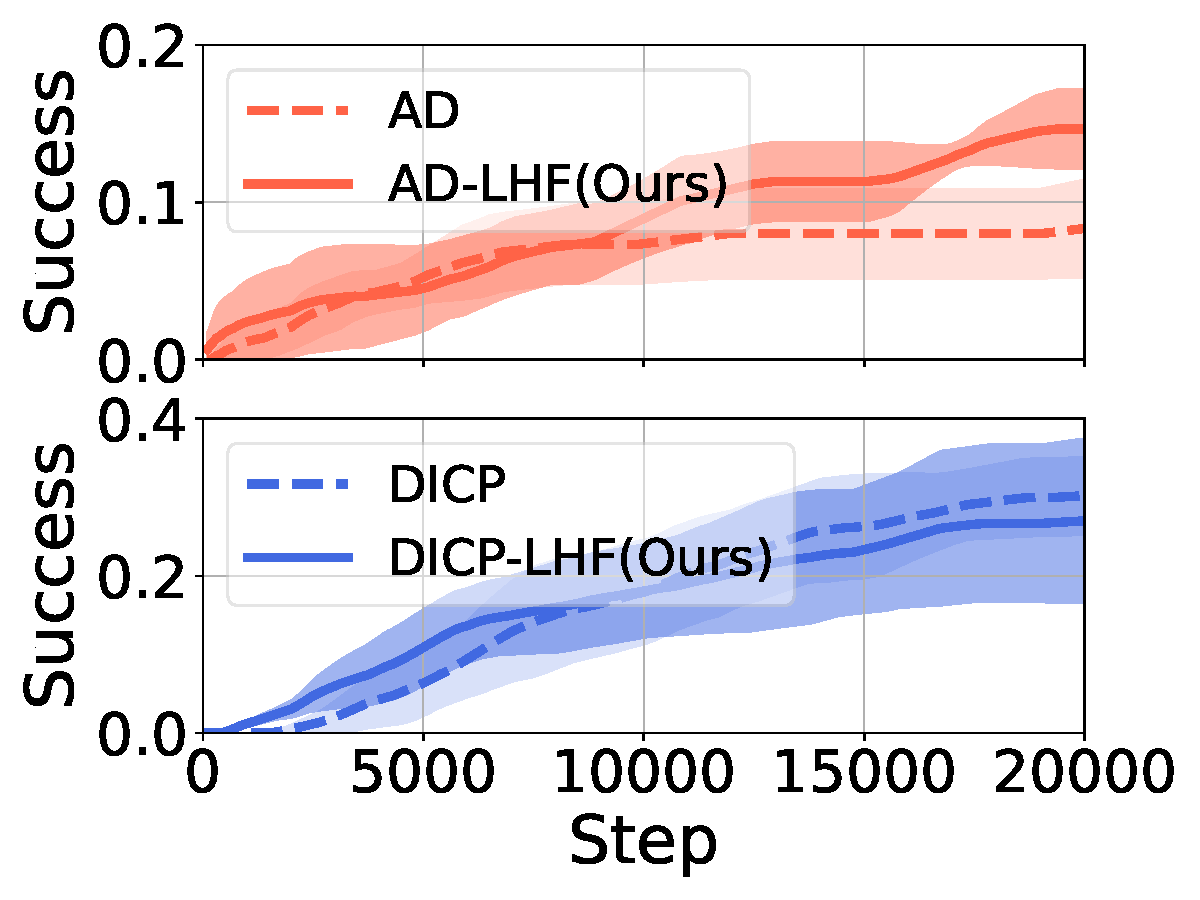
\includegraphics[width=1.0\columnwidth]{figures/push-v2_SAC.pdf}
	\end{minipage}
}
\!\!\!\!\!\!\!
\subfigure[Soccer]
{
	\begin{minipage}{0.25\linewidth}
	\centering 
	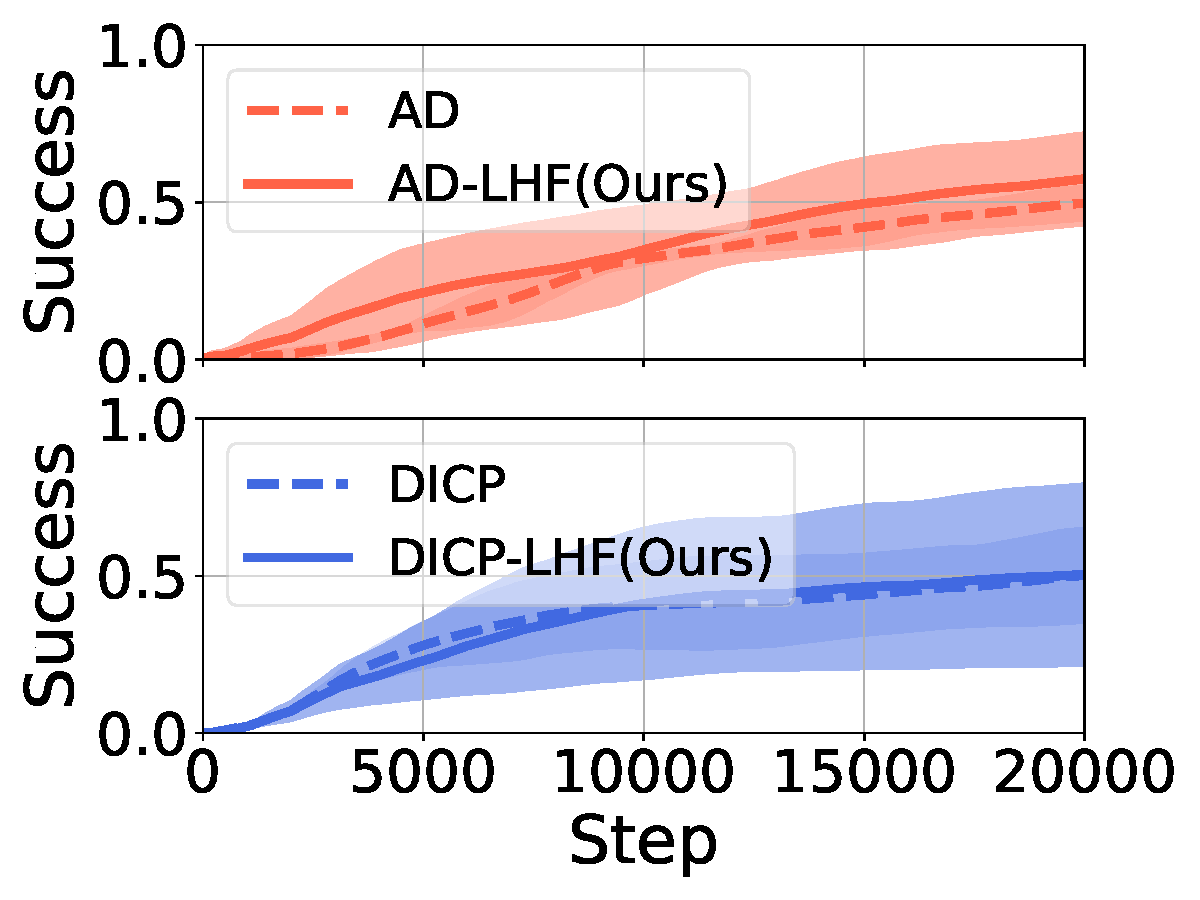
\includegraphics[width=1.0\columnwidth]{figures/soccer-v2_SAC.pdf}
	\end{minipage}
}
%
%
%
\caption{Learning curves of our LHF approach (solid lines) compared with original baselines (dashed lines) during the test. Each algorithm contains three independent runs with mean and std., provided with \textit{Meta-World-ML1} environments and datasets collected by SAC. The backbone algorithms include AD (red) and DICP (blue).}
\label{fig_sac_source_rl}
\end{figure}
%%%%%%%%%%%%%%%%








\section{Computing Infrastructure}
\label{Computing_Infrastructure}
All numerical experiments were conducted on a
workstation with
Intel\textregistered\ Core\texttrademark\ i9-14900KF CPU (32 threads),
and NVIDIA GeForce RTX 4090 GPU (24 GB), 64 GB RAM.


\section{Code}


The codes will be made available upon the publication of this work.
































% %%%%%%%%%%%%%%%%%%%%%%%%%%%%%%%%%%%%%%%%%%%%%%%%%%%%%%%%%%%%

% % \newpage
% \clearpage
% \section*{NeurIPS Paper Checklist}

% %%% BEGIN INSTRUCTIONS %%%
% The checklist is designed to encourage best practices for responsible machine learning research, addressing issues of reproducibility, transparency, research ethics, and societal impact. Do not remove the checklist: {\bf The papers not including the checklist will be desk rejected.} The checklist should follow the references and follow the (optional) supplemental material.  The checklist does NOT count towards the page
% limit. 

% Please read the checklist guidelines carefully for information on how to answer these questions. For each question in the checklist:
% \begin{itemize}
%     \item You should answer \answerYes{}, \answerNo{}, or \answerNA{}.
%     \item \answerNA{} means either that the question is Not Applicable for that particular paper or the relevant information is Not Available.
%     \item Please provide a short (1–2 sentence) justification right after your answer (even for NA). 
%    % \item {\bf The papers not including the checklist will be desk rejected.}
% \end{itemize}

% {\bf The checklist answers are an integral part of your paper submission.} They are visible to the reviewers, area chairs, senior area chairs, and ethics reviewers. You will be asked to also include it (after eventual revisions) with the final version of your paper, and its final version will be published with the paper.

% The reviewers of your paper will be asked to use the checklist as one of the factors in their evaluation. While "\answerYes{}" is generally preferable to "\answerNo{}", it is perfectly acceptable to answer "\answerNo{}" provided a proper justification is given (e.g., "error bars are not reported because it would be too computationally expensive" or "we were unable to find the license for the dataset we used"). In general, answering "\answerNo{}" or "\answerNA{}" is not grounds for rejection. While the questions are phrased in a binary way, we acknowledge that the true answer is often more nuanced, so please just use your best judgment and write a justification to elaborate. All supporting evidence can appear either in the main paper or the supplemental material, provided in appendix. If you answer \answerYes{} to a question, in the justification please point to the section(s) where related material for the question can be found.

% IMPORTANT, please:
% \begin{itemize}
%     \item {\bf Delete this instruction block, but keep the section heading ``NeurIPS Paper Checklist"},
%     \item  {\bf Keep the checklist subsection headings, questions/answers and guidelines below.}
%     \item {\bf Do not modify the questions and only use the provided macros for your answers}.
% \end{itemize} 
 

% %%% END INSTRUCTIONS %%%


% \begin{enumerate}

% \item {\bf Claims}
%     \item[] Question: Do the main claims made in the abstract and introduction accurately reflect the paper's contributions and scope?
%     \item[] \textbf{Answer:} \answerYes{}
%     \item[] \textbf{Justification:} The abstract and introduction clearly state the contributions of the proposed method (LHF), which match the experiments and findings reported in the paper. We outline the scope of our paper and include the main contributions and claims in the abstract and introduction, including details on what our method is and what settings we tested it in.
%     \item[] Guidelines:
%     \begin{itemize}
%         \item The answer NA means that the abstract and introduction do not include the claims made in the paper.
%         \item The abstract and/or introduction should clearly state the claims made, including the contributions made in the paper and important assumptions and limitations. A No or NA answer to this question will not be perceived well by the reviewers. 
%         \item The claims made should match theoretical and experimental results, and reflect how much the results can be expected to generalize to other settings. 
%         \item It is fine to include aspirational goals as motivation as long as it is clear that these goals are not attained by the paper. 
%     \end{itemize}

% \item {\bf Limitations}
%     \item[] Question: Does the paper discuss the limitations of the work performed by the authors?
%     \item[] \textbf{Answer:} \answerYes{}
%     \item[] \textbf{Justification:}
% Section~\ref{discussion_section} (\emph{Discussion}) includes a specific paragraph on limitations (e.g., no theoretical guarantees in the specific context of ICRL, and that LHF is not geared toward in-context safe RL).
%     \item[] Guidelines:
%     \begin{itemize}
%         \item The answer NA means that the paper has no limitation while the answer No means that the paper has limitations, but those are not discussed in the paper. 
%         \item The authors are encouraged to create a separate "Limitations" section in their paper.
%         \item The paper should point out any strong assumptions and how robust the results are to violations of these assumptions (e.g., independence assumptions, noiseless settings, model well-specification, asymptotic approximations only holding locally). The authors should reflect on how these assumptions might be violated in practice and what the implications would be.
%         \item The authors should reflect on the scope of the claims made, e.g., if the approach was only tested on a few datasets or with a few runs. In general, empirical results often depend on implicit assumptions, which should be articulated.
%         \item The authors should reflect on the factors that influence the performance of the approach. For example, a facial recognition algorithm may perform poorly when image resolution is low or images are taken in low lighting. Or a speech-to-text system might not be used reliably to provide closed captions for online lectures because it fails to handle technical jargon.
%         \item The authors should discuss the computational efficiency of the proposed algorithms and how they scale with dataset size.
%         \item If applicable, the authors should discuss possible limitations of their approach to address problems of privacy and fairness.
%         \item While the authors might fear that complete honesty about limitations might be used by reviewers as grounds for rejection, a worse outcome might be that reviewers discover limitations that aren't acknowledged in the paper. The authors should use their best judgment and recognize that individual actions in favor of transparency play an important role in developing norms that preserve the integrity of the community. Reviewers will be specifically instructed to not penalize honesty concerning limitations.
%     \end{itemize}

% \item {\bf Theory assumptions and proofs}
%     \item[] Question: For each theoretical result, does the paper provide the full set of assumptions and a complete (and correct) proof?
%     \item[] \textbf{Answer:} \answerNA{}
%     \item[] \textbf{Justification:}
% This work does not include any theoretical results.
%     \item[] Guidelines:
%     \begin{itemize}
%         \item The answer NA means that the paper does not include theoretical results. 
%         \item All the theorems, formulas, and proofs in the paper should be numbered and cross-referenced.
%         \item All assumptions should be clearly stated or referenced in the statement of any theorems.
%         \item The proofs can either appear in the main paper or the supplemental material, but if they appear in the supplemental material, the authors are encouraged to provide a short proof sketch to provide intuition. 
%         \item Inversely, any informal proof provided in the core of the paper should be complemented by formal proofs provided in appendix or supplemental material.
%         \item Theorems and Lemmas that the proof relies upon should be properly referenced. 
%     \end{itemize}

%     \item {\bf Experimental result reproducibility}
%     \item[] Question: Does the paper fully disclose all the information needed to reproduce the main experimental results of the paper to the extent that it affects the main claims and/or conclusions of the paper (regardless of whether the code and data are provided or not)?
% \item[] \textbf{Answer:} \answerYes{}
% \item[] \textbf{Justification:}
% We provide detailed pseudocode, diagrams, and extensive appendix sections that allow complete re-implementation. For example, Section~\ref{section_experiment} and Appendices provide environment details, data-collection procedures, hyperparameters for PPO and SAC, and the backbone ICRL algorithms. This information is sufficient to reproduce the experiments that support the main claims.
%     \item[] Guidelines:
%     \begin{itemize}
%         \item The answer NA means that the paper does not include experiments.
%         \item If the paper includes experiments, a No answer to this question will not be perceived well by the reviewers: Making the paper reproducible is important, regardless of whether the code and data are provided or not.
%         \item If the contribution is a dataset and/or model, the authors should describe the steps taken to make their results reproducible or verifiable. 
%         \item Depending on the contribution, reproducibility can be accomplished in various ways. For example, if the contribution is a novel architecture, describing the architecture fully might suffice, or if the contribution is a specific model and empirical evaluation, it may be necessary to either make it possible for others to replicate the model with the same dataset, or provide access to the model. In general. releasing code and data is often one good way to accomplish this, but reproducibility can also be provided via detailed instructions for how to replicate the results, access to a hosted model (e.g., in the case of a large language model), releasing of a model checkpoint, or other means that are appropriate to the research performed.
%         \item While NeurIPS does not require releasing code, the conference does require all submissions to provide some reasonable avenue for reproducibility, which may depend on the nature of the contribution. For example
%         \begin{enumerate}
%             \item If the contribution is primarily a new algorithm, the paper should make it clear how to reproduce that algorithm.
%             \item If the contribution is primarily a new model architecture, the paper should describe the architecture clearly and fully.
%             \item If the contribution is a new model (e.g., a large language model), then there should either be a way to access this model for reproducing the results or a way to reproduce the model (e.g., with an open-source dataset or instructions for how to construct the dataset).
%             \item We recognize that reproducibility may be tricky in some cases, in which case authors are welcome to describe the particular way they provide for reproducibility. In the case of closed-source models, it may be that access to the model is limited in some way (e.g., to registered users), but it should be possible for other researchers to have some path to reproducing or verifying the results.
%         \end{enumerate}
%     \end{itemize}


% \item {\bf Open access to data and code}
%     \item[] Question: Does the paper provide open access to the data and code, with sufficient instructions to faithfully reproduce the main experimental results, as described in supplemental material?
%     \item[] \textbf{Answer:}  \answerNA{}
%     \item[] \textbf{Justification:}
%     We will release our source code along with comprehensive instructions to facilitate the reproduction of all experimental results presented in this work upon publication.
%     \item[] Guidelines:
%     \begin{itemize}
%         \item The answer NA means that paper does not include experiments requiring code.
%         \item Please see the NeurIPS code and data submission guidelines (\url{https://nips.cc/public/guides/CodeSubmissionPolicy}) for more details.
%         \item While we encourage the release of code and data, we understand that this might not be possible, so “No” is an acceptable answer. Papers cannot be rejected simply for not including code, unless this is central to the contribution (e.g., for a new open-source benchmark).
%         \item The instructions should contain the exact command and environment needed to run to reproduce the results. See the NeurIPS code and data submission guidelines (\url{https://nips.cc/public/guides/CodeSubmissionPolicy}) for more details.
%         \item The authors should provide instructions on data access and preparation, including how to access the raw data, preprocessed data, intermediate data, and generated data, etc.
%         \item The authors should provide scripts to reproduce all experimental results for the new proposed method and baselines. If only a subset of experiments are reproducible, they should state which ones are omitted from the script and why.
%         \item At submission time, to preserve anonymity, the authors should release anonymized versions (if applicable).
%         \item Providing as much information as possible in supplemental material (appended to the paper) is recommended, but including URLs to data and code is permitted.
%     \end{itemize}


% \item {\bf Experimental setting/details}
%     \item[] Question: Does the paper specify all the training and test details (e.g., data splits, hyperparameters, how they were chosen, type of optimizer, etc.) necessary to understand the results?
% \item[] \textbf{Answer:} \answerYes{}
%     \item[] \textbf{Justification:} Section~\ref{section_experiment} and all Appendices disclose all relevant details, including dataset splits (e.g., pretraining vs.\ test environments), training hyperparameters, and the specific PPO/SAC setups. We also explain the rationale for choosing certain hyperparameters (like horizon length) in each environment.
%     \item[] Guidelines:
%     \begin{itemize}
%         \item The answer NA means that the paper does not include experiments.
%         \item The experimental setting should be presented in the core of the paper to a level of detail that is necessary to appreciate the results and make sense of them.
%         \item The full details can be provided either with the code, in appendix, or as supplemental material.
%     \end{itemize}

% \item {\bf Experiment statistical significance}
%     \item[] Question: Does the paper report error bars suitably and correctly defined or other appropriate information about the statistical significance of the experiments?
% \item[] \textbf{Answer:} \answerYes{}
%     \item[] \textbf{Justification:} In all plots in the paper, we display the mean across 3 independent runs along with shaded regions indicating the standard deviation. Each run uses a different random seed and environment shuffle, providing an honest measure of variability.

%     \item[] Guidelines:
%     \begin{itemize}
%         \item The answer NA means that the paper does not include experiments.
%         \item The authors should answer "Yes" if the results are accompanied by error bars, confidence intervals, or statistical significance tests, at least for the experiments that support the main claims of the paper.
%         \item The factors of variability that the error bars are capturing should be clearly stated (for example, train/test split, initialization, random drawing of some parameter, or overall run with given experimental conditions).
%         \item The method for calculating the error bars should be explained (closed form formula, call to a library function, bootstrap, etc.)
%         \item The assumptions made should be given (e.g., Normally distributed errors).
%         \item It should be clear whether the error bar is the standard deviation or the standard error of the mean.
%         \item It is OK to report 1-sigma error bars, but one should state it. The authors should preferably report a 2-sigma error bar than state that they have a 96\% CI, if the hypothesis of Normality of errors is not verified.
%         \item For asymmetric distributions, the authors should be careful not to show in tables or figures symmetric error bars that would yield results that are out of range (e.g. negative error rates).
%         \item If error bars are reported in tables or plots, The authors should explain in the text how they were calculated and reference the corresponding figures or tables in the text.
%     \end{itemize}

% \item {\bf Experiments compute resources}
%     \item[] Question: For each experiment, does the paper provide sufficient information on the computer resources (type of compute workers, memory, time of execution) needed to reproduce the experiments?
% \item[] \textbf{Answer:} \answerYes{}
%     \item[] \textbf{Justification:} We provide a summary of the computational resources used for our experiments in Appendix~\ref{Computing_Infrastructure}.
%     \item[] Guidelines:
%     \begin{itemize}
%         \item The answer NA means that the paper does not include experiments.
%         \item The paper should indicate the type of compute workers CPU or GPU, internal cluster, or cloud provider, including relevant memory and storage.
%         \item The paper should provide the amount of compute required for each of the individual experimental runs as well as estimate the total compute. 
%         \item The paper should disclose whether the full research project required more compute than the experiments reported in the paper (e.g., preliminary or failed experiments that didn't make it into the paper). 
%     \end{itemize}
    
% \item {\bf Code of ethics}
%     \item[] Question: Does the research conducted in the paper conform, in every respect, with the NeurIPS Code of Ethics \url{https://neurips.cc/public/EthicsGuidelines}?
%    \item[] \textbf{Answer:} \answerYes{}
%     \item[] \textbf{Justification:} We have reviewed the ethics guidelines and confirmed that our paper complies with the NeurIPS Code of Ethics.
%     \item[] Guidelines:
%     \begin{itemize}
%         \item The answer NA means that the authors have not reviewed the NeurIPS Code of Ethics.
%         \item If the authors answer No, they should explain the special circumstances that require a deviation from the Code of Ethics.
%         \item The authors should make sure to preserve anonymity (e.g., if there is a special consideration due to laws or regulations in their jurisdiction).
%     \end{itemize}


% \item {\bf Broader impacts}
%     \item[] Question: Does the paper discuss both potential positive societal impacts and negative societal impacts of the work performed?
% \item[] \textbf{Answer:} \answerNA{}
%     \item[] \textbf{Justification:} Our paper is foundation research and does not have a direct path to negative applications.

%     \item[] Guidelines:
%     \begin{itemize}
%         \item The answer NA means that there is no societal impact of the work performed.
%         \item If the authors answer NA or No, they should explain why their work has no societal impact or why the paper does not address societal impact.
%         \item Examples of negative societal impacts include potential malicious or unintended uses (e.g., disinformation, generating fake profiles, surveillance), fairness considerations (e.g., deployment of technologies that could make decisions that unfairly impact specific groups), privacy considerations, and security considerations.
%         \item The conference expects that many papers will be foundational research and not tied to particular applications, let alone deployments. However, if there is a direct path to any negative applications, the authors should point it out. For example, it is legitimate to point out that an improvement in the quality of generative models could be used to generate deepfakes for disinformation. On the other hand, it is not needed to point out that a generic algorithm for optimizing neural networks could enable people to train models that generate Deepfakes faster.
%         \item The authors should consider possible harms that could arise when the technology is being used as intended and functioning correctly, harms that could arise when the technology is being used as intended but gives incorrect results, and harms following from (intentional or unintentional) misuse of the technology.
%         \item If there are negative societal impacts, the authors could also discuss possible mitigation strategies (e.g., gated release of models, providing defenses in addition to attacks, mechanisms for monitoring misuse, mechanisms to monitor how a system learns from feedback over time, improving the efficiency and accessibility of ML).
%     \end{itemize}
    
% \item {\bf Safeguards}
%     \item[] Question: Does the paper describe safeguards that have been put in place for responsible release of data or models that have a high risk for misuse (e.g., pretrained language models, image generators, or scraped datasets)?
%     \item[] \textbf{Answer:} \answerNA{}
%     \item[] \textbf{Justification:} We do not scrape any data, nor do our models pose a high risk for misuse.
%     \item[] Guidelines:
%     \begin{itemize}
%         \item The answer NA means that the paper poses no such risks.
%         \item Released models that have a high risk for misuse or dual-use should be released with necessary safeguards to allow for controlled use of the model, for example by requiring that users adhere to usage guidelines or restrictions to access the model or implementing safety filters. 
%         \item Datasets that have been scraped from the Internet could pose safety risks. The authors should describe how they avoided releasing unsafe images.
%         \item We recognize that providing effective safeguards is challenging, and many papers do not require this, but we encourage authors to take this into account and make a best faith effort.
%     \end{itemize}

% \item {\bf Licenses for existing assets}
%  \item[] Question: Are the creators or original owners of assets (e.g., code, data, models), used in the paper, properly credited and are the license and terms of use explicitly mentioned and properly respected?
%     \item[] \textbf{Answer:} \answerYes{}
%     \item[] \textbf{Justification:} All prior work and assets are cited with proper attribution. For example, we cite the original sources for \textit{Meta-World} \cite{yu2020meta} and for Stable Baselines3 PPO/SAC \cite{stable-baselines3}, both of which are covered by standard open-source licenses. These references appear throughout the paper and in the bibliography.
%     \item[] Guidelines:
%     \begin{itemize}
%         \item The answer NA means that the paper does not use existing assets.
%         \item The authors should cite the original paper that produced the code package or dataset.
%         \item The authors should state which version of the asset is used and, if possible, include a URL.
%         \item The name of the license (e.g., CC-BY 4.0) should be included for each asset.
%         \item For scraped data from a particular source (e.g., website), the copyright and terms of service of that source should be provided.
%         \item If assets are released, the license, copyright information, and terms of use in the package should be provided. For popular datasets, \url{paperswithcode.com/datasets} has curated licenses for some datasets. Their licensing guide can help determine the license of a dataset.
%         \item For existing datasets that are re-packaged, both the original license and the license of the derived asset (if it has changed) should be provided.
%         \item If this information is not available online, the authors are encouraged to reach out to the asset's creators.
%     \end{itemize}

% \item {\bf New assets}
%     \item[] Question: Are new assets introduced in the paper well documented and is the documentation provided alongside the assets?
%     \item[] \textbf{Answer:} \answerNA{}
%     \item[] \textbf{Justification:} No new external assets are released; data are self-generated.
%     \item[] Guidelines:
%     \begin{itemize}
%         \item The answer NA means that the paper does not release new assets.
%         \item Researchers should communicate the details of the dataset/code/model as part of their submissions via structured templates. This includes details about training, license, limitations, etc. 
%         \item The paper should discuss whether and how consent was obtained from people whose asset is used.
%         \item At submission time, remember to anonymize your assets (if applicable). You can either create an anonymized URL or include an anonymized zip file.
%     \end{itemize}

% \item {\bf Crowdsourcing and research with human subjects}
%     \item[] Question: For crowdsourcing experiments and research with human subjects, does the paper include the full text of instructions given to participants and screenshots, if applicable, as well as details about compensation (if any)? 
%     \item[] \textbf{Answer:} \answerNA{}
%     \item[] \textbf{Justification:} No human subjects or crowdsourcing are involved in this work.
%     \item[] Guidelines:
%     \begin{itemize}
%         \item The answer NA means that the paper does not involve crowdsourcing nor research with human subjects.
%         \item Including this information in the supplemental material is fine, but if the main contribution of the paper involves human subjects, then as much detail as possible should be included in the main paper. 
%         \item According to the NeurIPS Code of Ethics, workers involved in data collection, curation, or other labor should be paid at least the minimum wage in the country of the data collector. 
%     \end{itemize}

% \item {\bf Institutional review board (IRB) approvals or equivalent for research with human subjects}
%     \item[] Question: Does the paper describe potential risks incurred by study participants, whether such risks were disclosed to the subjects, and whether Institutional Review Board (IRB) approvals (or an equivalent approval/review based on the requirements of your country or institution) were obtained?
%   \item[] \textbf{Answer:} \answerNA{}
%     \item[] \textbf{Justification:} We do not use any human-subject data or conduct user studies. Consequently, no IRB approval is required.

%     \item[] Guidelines:
%     \begin{itemize}
%         \item The answer NA means that the paper does not involve crowdsourcing nor research with human subjects.
%         \item Depending on the country in which research is conducted, IRB approval (or equivalent) may be required for any human subjects research. If you obtained IRB approval, you should clearly state this in the paper. 
%         \item We recognize that the procedures for this may vary significantly between institutions and locations, and we expect authors to adhere to the NeurIPS Code of Ethics and the guidelines for their institution. 
%         \item For initial submissions, do not include any information that would break anonymity (if applicable), such as the institution conducting the review.
%     \end{itemize}

% \item {\bf Declaration of LLM usage}
%     \item[] Question: Does the paper describe the usage of LLMs if it is an important, original, or non-standard component of the core methods in this research? Note that if the LLM is used only for writing, editing, or formatting purposes and does not impact the core methodology, scientific rigorousness, or originality of the research, declaration is not required.
%     %this research? 
% \item[] \textbf{Answer:} \answerNA{}
%     \item[] \textbf{Justification:} We don't use any LLM in the preparation of our paper.
%     \item[] Guidelines:
%     \begin{itemize}
%         \item The answer NA means that the core method development in this research does not involve LLMs as any important, original, or non-standard components.
%         \item Please refer to our LLM policy (\url{https://neurips.cc/Conferences/2025/LLM}) for what should or should not be described.
%     \end{itemize}

% \end{enumerate}












\end{document}